\chapter{Evoluční Algoritmy}

Evoluční algoritmy jsou metaheuristická optimalizační metoda odvozená z~teorie evoluce. Tato technika využívá pricipy darwinovské evoluce - selekci, mutaci a křížení k optimalizaci řešení. Tyto algoritmy jsou efektivní napříč různými problémy, protože mají jen málo předpokladů o povaze problému. Výpočetní náročnost vyplývající z vyhodnocování fitness funkce však může bránit jejich použití, ačkoli i jednodušší evoluční algoritmy mohou často řešit složité problémy.

Evoluční algoritmy mají v informatice kořeny od 40. let 20. století. První myšlenky o simulované evoluci předtavil Alan Turing v roce 1948 \cite{Turing1948}, prakticky se začaly používat v 60. letech 20. století. K tomuto oboru významně přispěli různí průkopníci z celého světa, včetně Johna Hollanda \cite{Holland1992}, nebo Johna Kozy \cite{Koza1994}. V~průběhu let se tento obor vyvinul a stal se předmětem několika vědeckých časopisů a specializovaných konferencí, jako jsou GECCO nebo CEC. 

\section{Zakládní definice}
V této sekci bychom chtěli definovat některé užitečné pojmy, ukázat základní komponenty evolučních algoritmů a zároveň vysvětlit, jakou hrají roli při návrhu a běhu algoritmu.

\subsection{Genom a Jedinec}
\emph{Genom} představuje jedno řešení pro daný problém. Je důležité zvolit vhodné kódování tohoto řešení. Holland si ve svém původním návrhu evolučního algoritmu představoval, že každé řešení bude kódované binárně \cite{Holland1992}, ale později se ukázalo, že je možné dosáhnout lepších výsledků, když kódováním reprezentujeme jakési stavební bloky daného řešení \cite{Jones1995Crossover}.

\emph{Jedincem} pak myslíme zastoupení genomu v populaci.

\subsection{Populace a Generace}
\emph{Populace} je seznam jedinců. Ze začátku běhu algoritmu populaci většinou naplníme jedinci s náhodnými genomy a postupnou aplikací genetických operátorů v~ní budeme evolvovat lepší a lepší řešení. \emph{Generace} představuje stav populace v~konkrétním čase.

\subsection{Genetické operátory}
\emph{Genetické operátory} jsou funkce, které můžeme aplikovat na jednoho a více jedinců nebo na celou populaci s cílem vybrat lepší jedince do další generace. Pomocí těchto operátorů můžeme vyvažovat exploraci a exploataci algoritmu a zároveň celou populaci směřovat k optimálnímu řešení \cite{EibenSmith2015}.

V kontextu genetických operátorů budeme často mluvit o \emph{rodičích} a \emph{potomcích}. Rodiči myslíme ty jedince, které se v populaci nachází před aplikací genetických operátorů, potomky pak ty, které se nachází po aplikaci, neboli v další generaci. 

\subsection{Křížení}
\emph{Křižení} je genetický operátor, kterým ze dvou nebo více jedinců (rodičů) můžeme vytvořit nového jedince (potomka), který strukturou připomíná oba (všechny) svoje rodiče. Tento proces je inspirován biologickou reprodukcí, kde potomci zdědí vlastnosti obou rodičů, což může vést k vyšší genetické variabilitě v populaci. Je důležité, aby nový potomek nebyl pouze náhodnou kombinací částí genů svých rodičů, ale aby křížení opravdu dávalo z hlediska struktury řešení smysl \cite{Jones1995Crossover}.

\subsection{Mutace}
\emph{Mutace} je genetický operátor, který může měnit náhodné části genomu. Od~křížení se liší hlavně tím, že je nezávislá na ostatních genomech v populaci. Význam mutací spočívá v udržení genetické diverzity populace, což je zásadní pro průzkum širšího prostoru řešení a předcházení předčasné konvergenci k suboptimálním řešením.

\subsection{Fitness}
\emph{Fitness} funkci budeme značit písmenem $f: G \rightarrow \R$, kde $G$ je množina všech možných genomů. Fitness nabízí měřitelnou kvalitu daného genomu a pomáhá algoritmu rozlišovat mezi více a méně vhodnými jedinci. Při návrhu fitness funkce je však nutné být opatrný, aby se předešlo běžným problémům, jako je předčasná konvergence nebo uváznutí v lokálních maximech. Není neobvyklé, že do fitness funkce je zahrnuto více různých komponent, které do výsledné hodnoty přispivají různými vahami. Tímto způsobem můžeme lépe rozlišit kvalitní řešení od těch nekvalitních a poskytnout algoritmu více informací pro efektivnější průzkum prostoru řešení. V praxi to může znamenat, že vedle hlavního kritéria, jako je například výkon nebo efektivita, mohou být do fitness funkce zahrnuty i sekundární kritéria, jako je cena, estetičnost nebo další metaheuristiky.

V problémech, které budeme chtít řešit evolučními algoritmy, se funkci $f$ obvykle snažíme maximalizovat. Jinými slovy, hledáme takový genom $g^* \in G$, že 
$$g^* = argmax_{g \in G} f(g)$$

\subsection{Selekce}
\emph{Selekce}, nebo také environmentální selekce, je genetický operátor, který simuluje proces přírodního výběru. Tento operátor přiřazuje jednotlivým jedincům jejich schopnosti přežívat a reprodukovat se na základě jejich fitness. Ti nejúspěšnější jedinci jsou vybíráni pro reprodukci, zatímco ti méně úspěšní jsou buď eliminováni nebo mají menší šanci přispět svými geny do další generace. Díky selekci se algoritmus soustředí na oblasti vyhledávacího prostoru s vysokým potenciálem, což vede k rychlejší a konvergenci k optimálním řešením. 

V kontextu selekce se často mluví o $(\mu + \lambda)$ a $(\mu, \lambda)$ strategiích pro selekci. 

\emph{$(\mu + \lambda)$ selekce} spočívá v tom, že z $\mu$ rodičů generujeme $\lambda$ potomků. Tyto potomky následně spojíme s původními rodiči a z této kombinované skupiny vybereme nejlepších $\mu$ jedinců pro další generaci. Tento přístup zajišťuje zachování nejlepších genetických vlastností z předešlých generací a poskytuje pojistku proti ztrátě kvalitních genů v případě, že nová generace by byla průměrně horší než její předchůdce \cite{EibenSmith2015}.

Na druhou stranu, \emph{$(\mu, \lambda)$ selekce} vychází z principu, kde $\mu$ rodičů generuje $\lambda$ potomků, ale pouze tito potomci postupují do další generace, což znamená úplné nahrazení původní populace. Tento proces, při němž jsou všichni rodiče nahrazení, pomáhá efektivněji překonávat lokální minima prostoru řešení, což je obzvláště cenné v situacích, kde prostor řešení obsahuje mnoho lokálních minim \cite{EibenSmith2015}.

Jako selekci nejčastěji používáme \emph{ruletovou selekci}, nebo \emph{turnajovou selekci}. Při ruletové selekci jedince $g_a$ vybere další generace s pravděpodobností $\frac{f(g_a)}{\sum_g f(g)}$. Při turnajové selekci vybereme náhodně $k$ jedinců z popupulace (většinou $k = \{2,3,5,10\}$). Z těchto $k$ jedinců postupuje do další populace pouze ten nejlepší.

\section{Evoluční algoritmus}

Příklad jednoduchého evolučního algoritmu může můžeme vidět v~algoritmu 1 \ref{alg:1}.

\begin{algorithm}
\caption{Jednoduchý evoluční algoritmus}
\begin{algorithmic}[1] 
\Function{EA}{Selekce, Křížení, Mutace, Fitness}
	\State $p \gets \mbox{náhodně inicializujeme populaci}$
    \State $f \gets Fitness(p_1), \dots, Fitness(p_n)$ \Comment{ohodnotíme fitness pro každého jedince}
	\While{$\mbox{není dosaženo zastavovací kriterium}$}
		\State $p \gets \mbox{Selekce}(p, f)$
		\State $p \gets \mbox{Křížení}(p)$
		\State $p \gets \mbox{Mutace}(p)$
        \State $f \gets \mbox{Fitness}(p_1), \dots, Fitness(p_n)$
    \EndWhile
    \State Vrátíme nejlepšího jedince z $p$
\EndFunction
\label{alg:1}
\end{algorithmic}
\end{algorithm}


\section{Příklad}

V této části bychom chtěli ukázat, jak lze navrhnout evoluční algoritmus pro řešení některých vybraných netriviálních problémů.

\subsection{Problém batohu} \label{batoh}

Problém batohu je generalizace mnoha industriálních problémů \cite{EibenSmith2015}. Představme si, že se balíme třeba na několikadenní túru do hor a s sebou bychom si chtěli zabalit batůžek. Chtěli bychom s sebou mít co nejužitečnější věci, ale zároveň si nemůžeme vzít všechno, protože bychom to neunesli. Problém batohu spočívá v tom, jak si vybrat věci, které si s sebou zabalíme, tak abychom maximalizovali užitek a zároveň se vešli do našeho stanoveného limitu.

Formálněji se tento problém definuje následovně. Je dána množina $n$ předmětů s hmotnostmi $h_1, \dots, h_n \in \N$, cenami $c_1, \dots, c_n \in \N$ a maximální hmotnost $H \in \N$. Hledáme takovou podmnožinu $p \subseteq \{1, \dots n\}$, pro kterou platí, že $\sum_{i \in P} h_i \leq H$ a zároveň $\sum_{i \in P} c_i$ je co největší.

Jako ilustrační řešení tomuto problému jsme navrhli tyto evoluční operátory a reprezentace:
\begin{itemize}
    \item Gen bude řetězec $\alpha \in \{0,1\}^n$, kde $\alpha_i$ ($i$-tý prvek z řetězce) značí, zda jsme se rozhodli vybrat $i$-tý prvek do množiny $p$ nebo ne.
    \item Jako selekci jsme zvolili turnajovou selekci.
    \item Jako mutaci jsme zvolili jednobodové křížení. To v praxi znamená, že nejdříve vybereme náhodný sdílený pro oba rodiče. Potomek pak zdědí z jednoho rodiče část řetězce před tímto bodem a z druhého část za ním. 
    \item Fitness funkce $f$ v tomto případě bude $f(\alpha) = \sum_{i=1}^n \alpha_i \cdot c_i$ pokud $\sum_{i=1}^n \alpha_i \cdot h_i < W$ jinak $0$
\end{itemize}

Výsledky běhu takového algoritmu můžeme vidět na~obrázku \ref{exp:1}

\chapter{Experimenty}

V následující sekci ukážem několik experimentů, které jsme provedli s pomocí naší implementace. Experimenty budou vždy porovnávat několik hyper parametrů evolučního algoritmu a graficky ukážou fitness nejlepšího nalezeného jedince v závislosti na počtu vyhodnocení fitness funkce. Kromě ukázky z batohem pokaždé ukážeme nalevo minimální vzdálnost od cíle a naprava cenu mostu. Jako prostředí simulace jsme zvolili vždy pouze $1.$ úroveň. Pro každý experiment a každou zmíněnou kombinaci hypermarametrů jsme provedli $5$ běhu a jejich výsledek zprůměrovali. Na obrázcích jsme tak znázornili také $95\%$ konfideční interval. Všechny experimenty jsme provedli na procesoru \texttt{AMD Ryzen 5 4500U with Radeon Graphics}. Vyhodnocování fitness jsme paralelizovali na všech $6$ jádrech procesoru.

\section{Jednoduchý příklad s batohem}

Experiment demonstruje výsledky běhu jednoduchého evolučního algoritmu na známém problému batohu, jak bylo představeno v sekci o problému batohu \ref{batoh}. Výsledky tohoto experimentu jsou prezentovány na obrázku \ref{exp:1}. Celková doba běhu jednoho experimentu byla přibližně $1$ minuta.

Z výsledků můžeme vidět, že běh poměrně rychle zkonvegroval. Už po $50$ generacích nelze pozorovat téměř žádné zlepšení. Zda jsem našli doopravdy optimální řešení bohužel nemužeme ověřit.

\begin{figure}[p]\centering
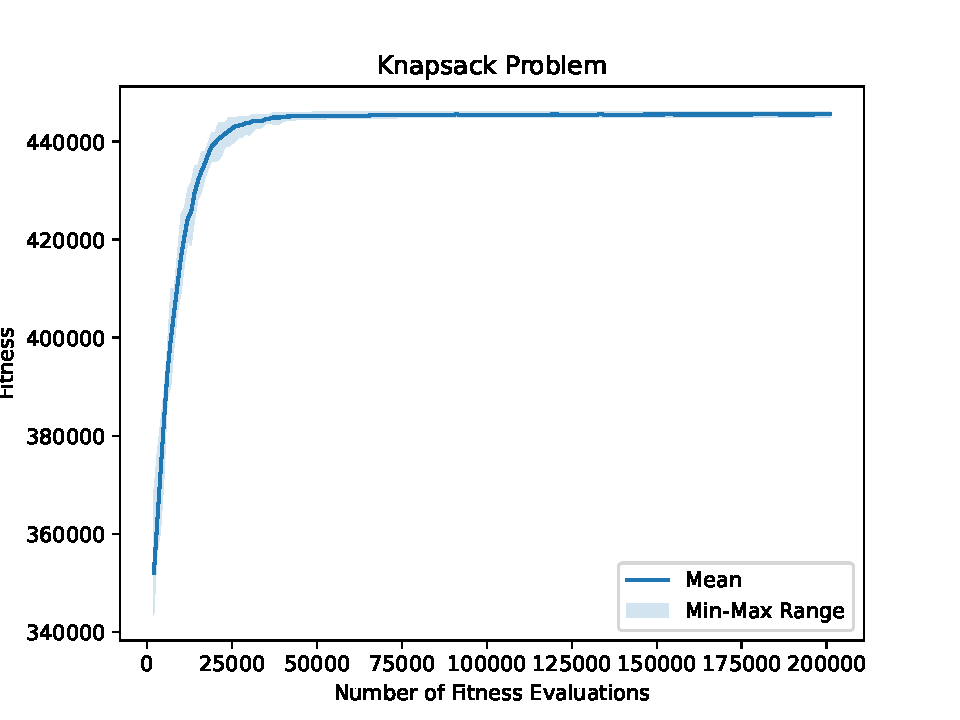
\includegraphics{img/knap}
\caption{Fitness nejlepšího jedince v závislosti na počtu vyhodnocení fitness funkce. Průměr $5$ běhů s $95\%$ konfidenčním intervalem. Velikost populace=$1000$, počet generací=$200$, p. mutace=$1/n$, p. křížení=$1$}
\label{exp:1}

\end{figure}


\section{Naivní přístup}

V tomto experimetu chceme ukázat, jakých výsledků lze dosáhnout pomocí jednoduchého kódování jedince. Z podstaty experimentu jsme se rozhodli vyzkoušet pouze jednu sadu hyperparametrů. Výsledek můžeme vidět na obrázku \ref{exp:2}. Doba jednoho běhu byla přibližně $11$ minut.

I přes jednoduchost našeho kódování se nám podařilo najít obstojný most. Tento postup bohužel ale vždy příliš brzy zkonverguje a tak se nám nedaří úroveň vyřešit.

\begin{figure}[p]\centering
\includegraphics[width=\linewidth]{img/simple}
\caption{Fitness nejlepšího jedince s jednoduchým kódováním v závislosti na počtu vyhodnocení fitness funkce. Nalevo minimální vzdálenost, napravo cena mostu. Průměr $5$ běhů s $95\%$ konfidenčním intervalem. Velikost populace=$250$, počet generací=$200$, p. mutace=$1/n$, p. křížení=$1$, délka jedince=$20$}
\label{exp:2}
\end{figure}


\section{Různé rozměry populace} \label{sizes}

Zkoumali jsme vliv různých kombinací velikosti populace a počtu generací na výkon algoritmu. Pro kódování jedinců jsme použili polární kódování. Výsledky jsou zobrazeny na obrázku \ref{exp:3}. Doba trvání jednoho běhu byla přibližně $11$ minut.

Z výsledků lze odvodit, že lepší fitness můžeme dosáhnout tím, že zvýšíme počet generací na úkor velikosti populace.

\begin{figure}[p]\centering
\includegraphics[width=\linewidth]{img/polar-pop}
\caption{Fitness nejlepšího jedince s polárním kódováním v závislosti na počtu vyhodnocení fitness funkce. Nalevo minimální vzdálenost, napravo cena mostu. Průměr $5$ běhů s $95\%$ konfidenčním intervalem. Velikost populace značená \emph{size}, počet generací značný \emph{gens}, p. mutace=$1/n$, p. křížení=$1$}
\label{exp:3}
\end{figure}

\section{Různé délky jedince}

Experimentovali jsme s různými délkami genomu pro jedince s polárním kódováním. Výsledky tohoto experimentu můžeme vidět na obrázku \ref{exp:35}. Délka běhu se lišila v závislosti na délce genomu, ale nepřesáhla $15$ minut.

Výsledky tohoto experimentu poukazují na důležitost výběru délky genomu jedince. Příliš krátký genom má za následek nedostatečnou schopnost jedince konstruovat kvalitní řešení, zatímco nadměrná délka vede k nadměrné hmotnosti a zhroucení celého mostu.

\begin{figure}[p]\centering
\includegraphics[width=\linewidth]{img/polar-len}
\caption{Fitness nejlepšího jedince s polárním kódováním v závislosti na počtu vyhodnocení fitness funkce. Nalevo minimální vzdálenost, napravo cena mostu. Průměr $5$ běhů s $95\%$ konfidenčním intervalem. Velikost populace=$250$, počet generací=$200$, p. mutace=$1/n$, p. křížení=$1$, délka jedince značí \emph{l}}
\label{exp:35}
\end{figure}

\section{Vylepšená fitness funkce}

Cílem tohoto experimentu je prozkoumat, zda vylepšená fintess funkce může zlepšít celkový výsledek algoritmu. Zkusili jsme několik různých vah $\alpha, \beta$ pro penalizace ve fitness funkci pro jedince s polárním kódováním. Výsledek toho experimenty můžeme vidět na obrázku \ref{exp:4}. Doba jednoho běhu byla přibližně $11$ minut.

Bylo překvapivé, že náš návrh fitness funkce s penalizacemi nepomohl nalezení lepšího mostu. Z výsledků experimentů se zdá, že algoritmus místo toho, optimalizoval strukturu mostu, přestane úplně most stavit. Docílí se tak minimální penalizace a tudíž i lepši fitness a předčasně zkonvergujeme do lokálního minima. 

\begin{figure}[p]\centering
\includegraphics[width=\linewidth]{img/impolar}
\caption{Fitness nejlepšího jedince s polárním kódováním a vylepšenou fitness funkcí v závislosti na počtu vyhodnocení fitness funkce. Nalevo minimální vzdálenost, napravo cena mostu. Průměr $5$ běhů s $95\%$ konfidenčním intervalem. Velikost populace=$250$, počet generací=$200$, p. mutace=$1/n$, p. křížení=$1$, délka jedince=$20$, parametry $\alpha, \beta$ značí \emph{alpha, beta}}
\label{exp:4}
\end{figure}


\section{Populace s elitismem} 

V tomto experimentu jsme vyzkoušeli jaký vliv má elitismus na běh algoritmu. Zkusili jsme několik úrovní elitismu pro jedince s polárním kódováním, jejich rozdíly můžme vidět na obrázku \ref{exp:5}. Doba jednoho běhu byla přibližně $11$ minut.

V tomto experimentu si můžeme všimnout, že elitismus tolik nepomáhá. Zajímavé je si všimnout i toho, že pokud nastavíme sílu elitismu vysoko, můžeme dosáhnout ještě lepších výsledků než bez elitismu. Tím se nám znovu potvrzuje náš závěr z experimentu \ref{sizes}, že můžeme dosáhnout lepší když budeme upřednostňovat eploataci.

\begin{figure}[p]\centering
\includegraphics[width=\linewidth]{img/elit}
\caption{Fitness nejlepšího jedince s polárním kódováním v závislosti na počtu vyhodnocení fitness funkce. Nalevo minimální vzdálenost, napravo cena mostu. Průměr $5$ běhů s $95\%$ konfidenčním intervalem. Velikost populace=$250$, počet generací=$200$, p. mutace=$1/n$, p. křížení=$1$, sílu elitismu značí $elit$}
\label{exp:5}
\end{figure}


\section{Ztěžující se fitness} \label{inc}

V následující experimentu vyzkoušíme, zda pomáhá postupné zvyšování obtížnosti problému. Počáteční vzdělenost břehů je nastavena na $10\%$ původní vzdálenosti. Vyzkoušeli jsme různé hranice průměrné fitness populace nutné na zvýšení obtížnosti. Také jsme zkusily různé velikosti kroků ztěžování. Použili jsme polární kódování jedince. Výsledek tohoto experimentu můžeme vidět na obrázke \ref{exp:6}. Doba jednoho běhu byla přibližně $11$ minut.

Bohužel se nám touto metodou nepodařil dosáhnout požadovaných výsledků. Z podstaty metody ale můžeme odvodit, že algoritmus nestihnul zkonvergovat k suboptimálnímu řešení, takže je možné, že kdybychom měli k dispozici více výpočetního času, mohli bychom mnohem lepších řešení.

\begin{figure}[p]\centering
\includegraphics[width=\linewidth]{img/inc}
\caption{Fitness nejlepšího jedince s polárním kódováním v závislosti na počtu vyhodnocení fitness funkce. Nalevo minimální vzdálenost, napravo cena mostu. Průměr $5$ běhů s $95\%$ konfidenčním intervalem. Velikost populace=$250$, počet generací=$200$, p. mutace=$1/n$, p. křížení=$1$, hranice pro zvýšení obtížnosti značí \emph{avg}, velikost kroku \emph{increase}}
\label{exp:6}
\end{figure}

\section{Grafové kódování}

Několik následující experimentů budou zkoumat efektivitu algoritmu s jedinci, kteří použivají grafové kódování. Nejdříve jsme zkoumali, jaký vliv má počet vrcholů na kvalitu jedinců. Výsledky experimentu jsou zobrazeny na obrázku \ref{exp:7}. Doba běhu se lišila v závislosti na délce jedince, ale nebyla delší než $21$ minut.

Je těžké z výsledků tohoto experimentu něco odvodit. Počet hran v genomu jedince se můžem mutacemi měnit tak na počátečním počtu vrcholů (tudíž i hran) příliš nezáleží.

\begin{figure}[p]\centering
\includegraphics[width=\linewidth]{img/graph}
\caption{Fitness nejlepšího jedince s grafovým kódování v závislosti na počtu vyhodnocení fitness funkce. Nalevo minimální vzdálenost, napravo cena mostu. Průměr $5$ běhů s $95\%$ konfidenčním intervalem. Velikost populace=$250$, počet generací=$200$, p. mutace vrcholu=$1/n$, p.mutace hrany = $1/n$, p. křížení=$1$, \emph{nodes} značí různé počty použitých vrcholů}
\label{exp:7}
\end{figure}


\section{Grafové kódování a stěžující se fitness}

Tento experiment rozšiřuje předchozí testování grafového kódování o postupné ztěžování problému během evoluce. Cílem bylo zjistit, zda kombinace grafového kódování a postupného zvyšování obtížnosti může vést k robustnější adaptaci jedinců na složitější úkoly. Výsledek tohoto experimentu můžeme vidět na obrázku \ref{exp:8}. Doba jednoho běhu byla přibližně $20$ minut.

Z tohoto experimentu můžeme odvodit podobné závéry jako z experimentu~\ref{inc}. \xxx{závěr tohoto experimentu musím dopsat až doběhne}

\begin{figure}[p]\centering
\includegraphics[width=\linewidth]{img/graph-inc}
\caption{Fitness nejlepšího jedince s grafovým kódování v závislosti na počtu vyhodnocení fitness funkce. Nalevo minimální vzdálenost, napravo cena mostu. Průměr $5$ běhů s $95\%$ konfidenčním intervalem. Velikost populace=$250$, počet generací=$200$, p. mutace=$1/n$, p. křížení=$1$, hranice pro zvýšení obtížnosti značí \emph{avg}, velikost kroku \emph{increase}}
\label{exp:8}
\end{figure}


\section{Lepší inicializace jedince}

Poslední experiment se zaměřuje na vliv vylepšené inicializace jedinců s grafovým kódování na celkový výkon evolučního algoritmu. Vyzkoušeli jsme různé hodnoty $\omega$. Výsledky jsou ilustrovány na obrázku \ref{exp:9}. Doba běhu se mírně lišila v závislosti na metodě inicializace, ale průměrně trvala 10 minut.

Tento experiment ukazuje, že tímto způsobem inicializace vpodstatě těžkou část problému, tedy dostat vozidlo z jedné strany na druhou, vyřeším neoptimální návrhem. Algoritmu pak zbývá pouze tento návrh lehce modifikovat mutacemi a křížením, což se jeví jako mnohem lepší postup, než se nejprve snažit najít optimální strukturu mostu. 

\begin{figure}[p]\centering
\includegraphics[width=\linewidth]{img/init}
\caption{Fitness nejlepšího jedince s grafovým kódování a vylepšenou inicializací v závislosti na počtu vyhodnocení fitness funkce. Nalevo minimální vzdálenost, napravo cena mostu. Průměr $5$ běhů s $95\%$ konfidenčním intervalem. Velikost populace=$250$, počet generací=$200$, p. mutace vrcholu=$1/n$, p.mutace hrany = $1/n$, p. křížení=$1$, \emph{omega} značí různé hodnoty $\omega$}
\label{exp:9}
\end{figure}


\begin{figure}[p]\centering
\includegraphics[width=\linewidth]{img/comp}
\caption{Porovnání různých kódování jedinců. \emph{t} značí typ jedince}
\label{zaver:1}
\end{figure}


\section{Přenesení do Poly Bridge}

V tomto exeperimentu ukážeme, jak nejlepší nalezená řešení pomocí evolučních algoritmu fungují ve hře. Na obrázcích \ref{exp:lvl1}, \ref{exp:lvl2}, \ref{exp:lvl3} a \ref{exp:lvl4} můžeme vidět porovnání nalezeních řešení v simulaci, ve hře a řešení navrhnutá člověkem. V tabluce \ref{tab:2} můžeme vidět, zda se nám úroveň podařilo vyřešit evolučním algoritmem a cenu navrženého mostu. Pro hledání řešení jsme pro všechny úrovně zvolili grafové kódování jedince s vylepšenou inicializací ($\omega=1$), velikostí populace $size=500$, počet generací $gens=1000$ s nízkým elitismem $0.02$. Takto nastavený algorimtus jsme pro každou úroveň zopakovali $5$krát a vybrali nejlepší řešení. Doba jednoho běhu byla zrhuba $25$ minut.

Evolučním algoritmem se nám podařilo vyřešeit $3$ ze $4$ úrovní, u dvou znich algoritmus navrhnul levnější řešení než člověk.

\begin{table}[b!]
\centering
\begin{tabular}{lccc}
\toprule
\textbf{Úroveň} & \textbf{Vyřešeno algoritmem} & \textbf{Cena \$} & \textbf{Cena lidského řešení \$} \\
\midrule
\emph{Úroveň 1} & Ano &  4133 & 3954 \\
\emph{Úroveň 2} & Ano &  3262 & 5752 \\
\emph{Úroveň 3} & Ano &  5544 & 5736 \\
\emph{Úroveň 4} & Ne  &  3788 & 4821 \\
\bottomrule
\end{tabular}
\caption{Ceny mostů navržených evolučním algoritme v porovnání s lidským řešením}
\label{tab:2}
\end{table}


\begin{figure}[ht]
    \centering
    \begin{minipage}{0.32\textwidth}
        \centering
        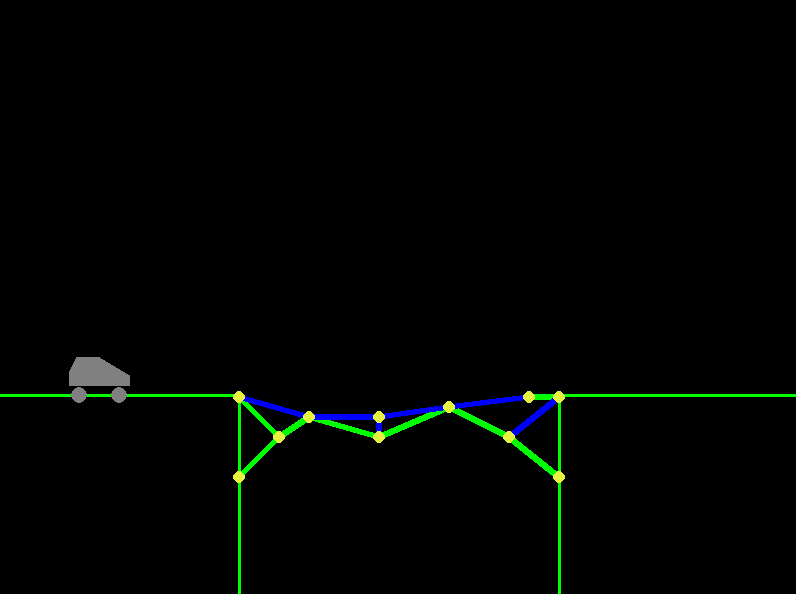
\includegraphics[width=\linewidth]{img/lvl1-sim-ea}
    \end{minipage}\hfill
    \begin{minipage}{0.32\textwidth}
        \centering
        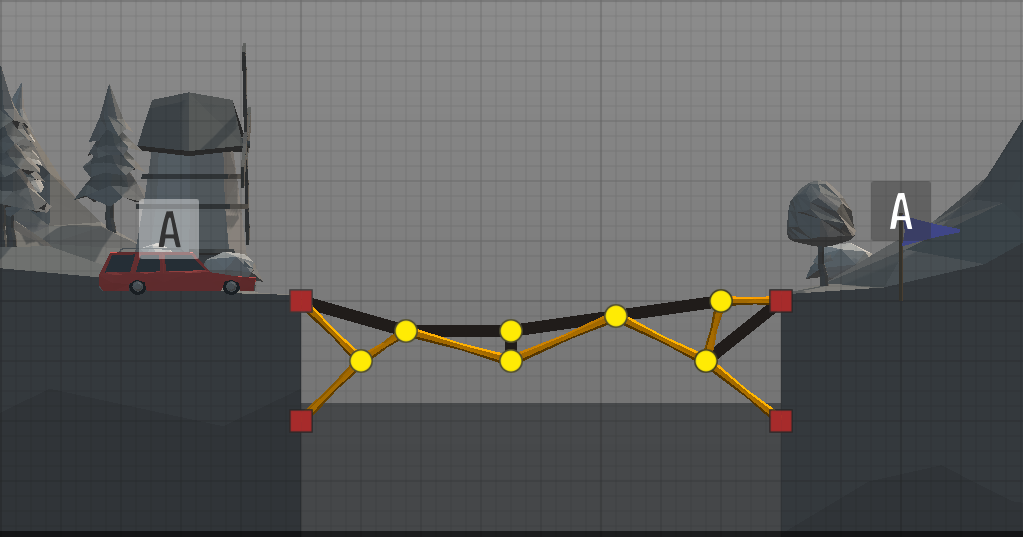
\includegraphics[width=\linewidth]{img/lvl1-poly-ea}
    \end{minipage}
    \begin{minipage}{0.32\textwidth}
        \centering
        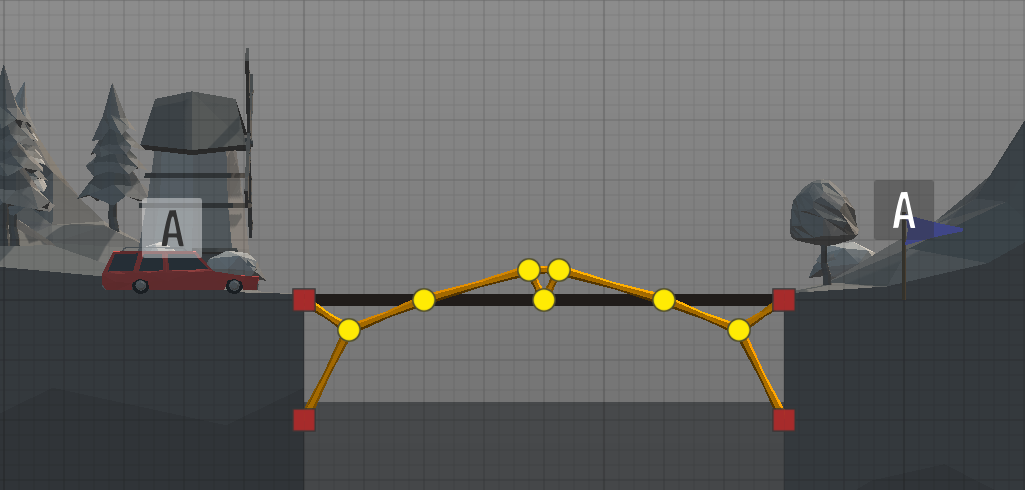
\includegraphics[width=\linewidth]{img/lvl1-poly-human}
    \end{minipage}
    \caption{Řešení první úrovně navrhnuté evolučním algoritmem. Nalevo je řešení zobrazené v simulaci, uprostřed ve hře, napravo řešení navrhnuté člověkem}
    \label{exp:lvl1}
\end{figure}

\begin{figure}[ht]
    \centering
    \begin{minipage}{0.32\textwidth}
        \centering
        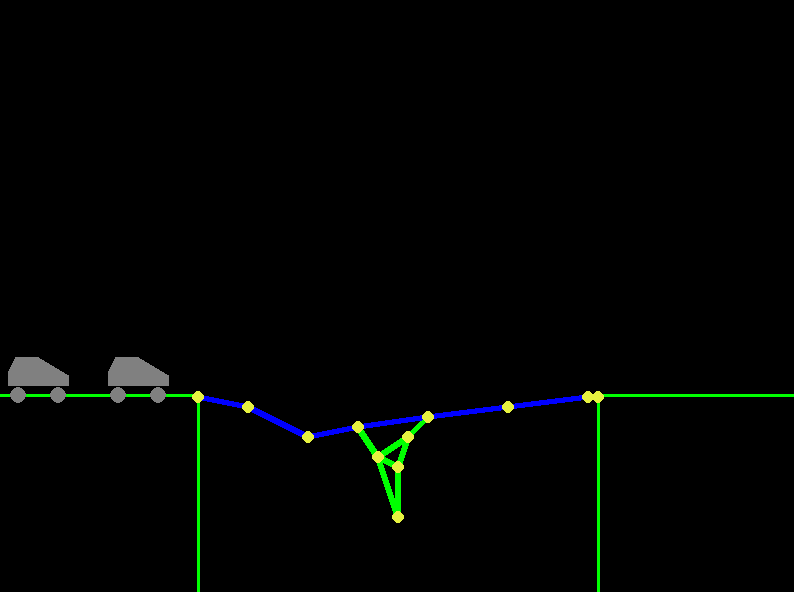
\includegraphics[width=\linewidth]{img/lvl2-sim-ea}
    \end{minipage}\hfill
    \begin{minipage}{0.32\textwidth}
        \centering
        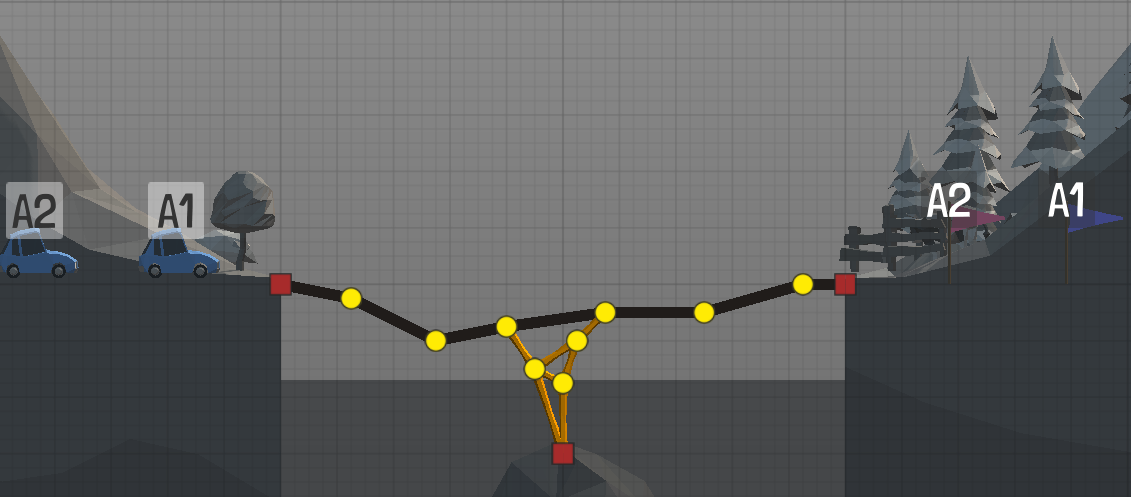
\includegraphics[width=\linewidth]{img/lvl2-poly-ea}
    \end{minipage}
    \begin{minipage}{0.32\textwidth}
        \centering
        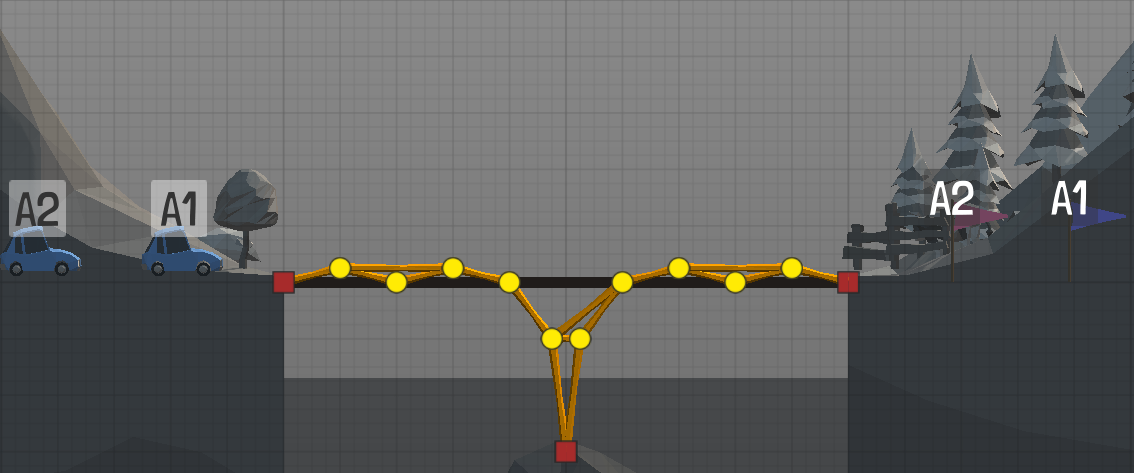
\includegraphics[width=\linewidth]{img/lvl2-poly-human}
    \end{minipage}
    \caption{Řešení druhé úrovně navrhnuté evolučním algoritmem. Nalevo je řešení zobrazené v simulaci, uprostřed ve hře, napravo řešení navrhnuté člověkem}
    \label{exp:lvl2}
\end{figure}

\begin{figure}[ht]
    \centering
    \begin{minipage}{0.32\textwidth}
        \centering
        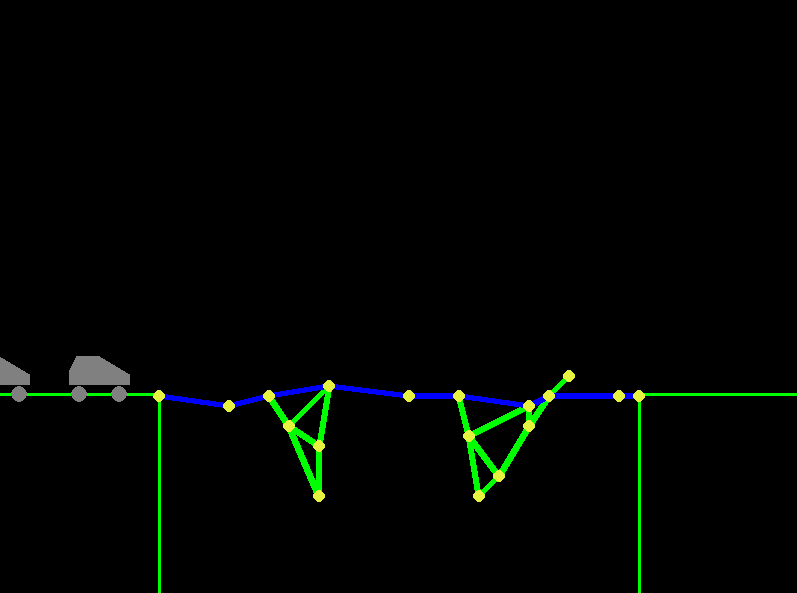
\includegraphics[width=\linewidth]{img/lvl3-sim-ea}
    \end{minipage}\hfill
    \begin{minipage}{0.32\textwidth}
        \centering
        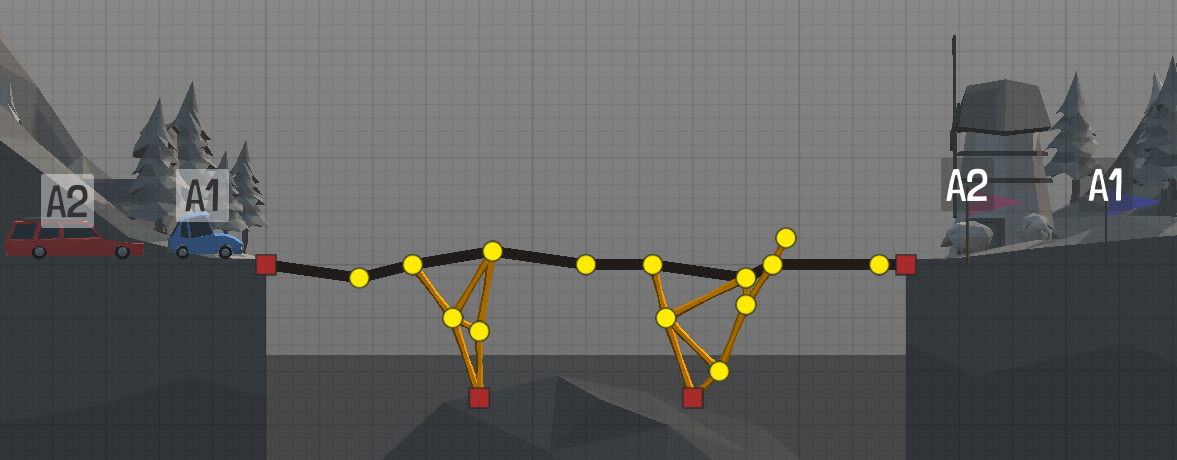
\includegraphics[width=\linewidth]{img/lvl3-poly-ea}
    \end{minipage}
    \begin{minipage}{0.32\textwidth}
        \centering
        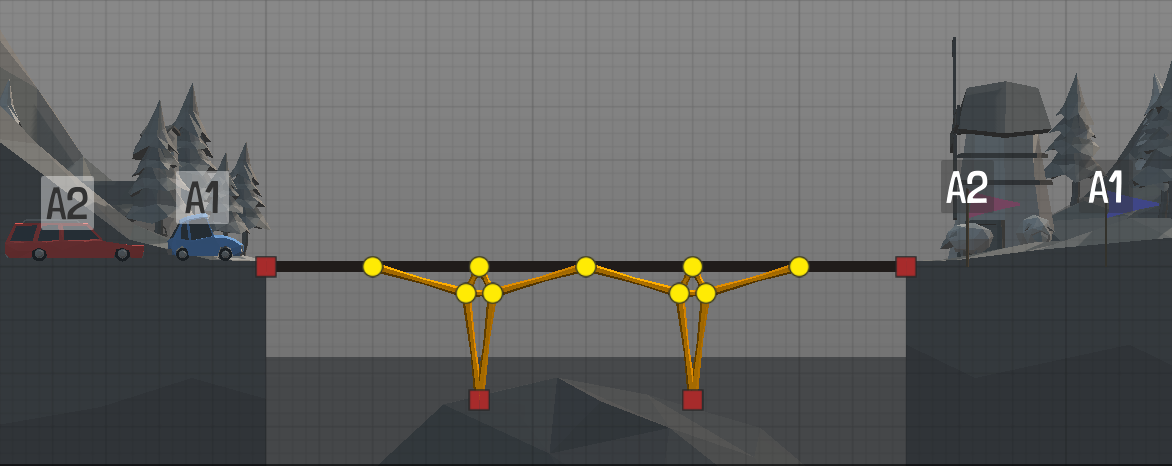
\includegraphics[width=\linewidth]{img/lvl3-poly-human}
    \end{minipage}
    \caption{Řešení třetí úrovně navrhnuté evolučním algoritmem. Nalevo je řešení zobrazené v simulaci, uprostřed ve hře, napravo řešení navrhnuté člověkem}
    \label{exp:lvl3}
\end{figure}

\begin{figure}[ht]
    \centering
    \begin{minipage}{0.32\textwidth}
        \centering
        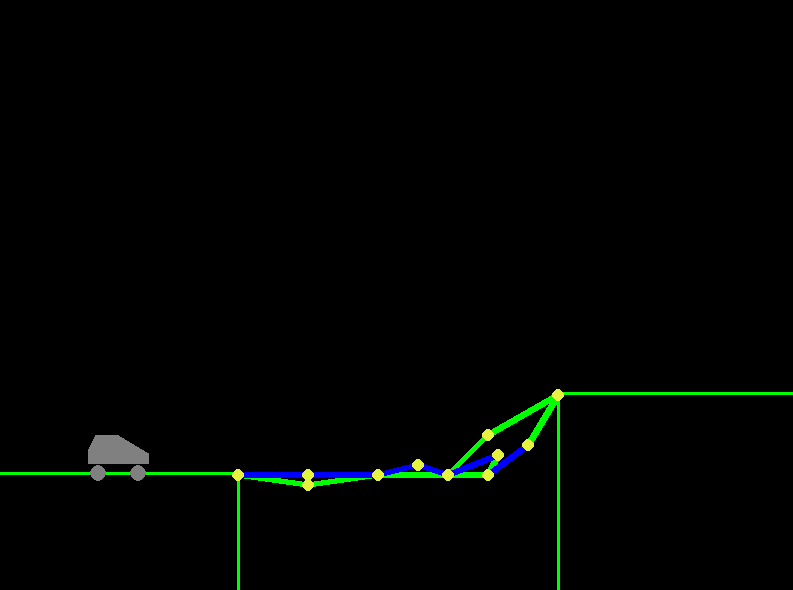
\includegraphics[width=\linewidth]{img/lvl4-sim-ea}
    \end{minipage}\hfill
    \begin{minipage}{0.32\textwidth}
        \centering
        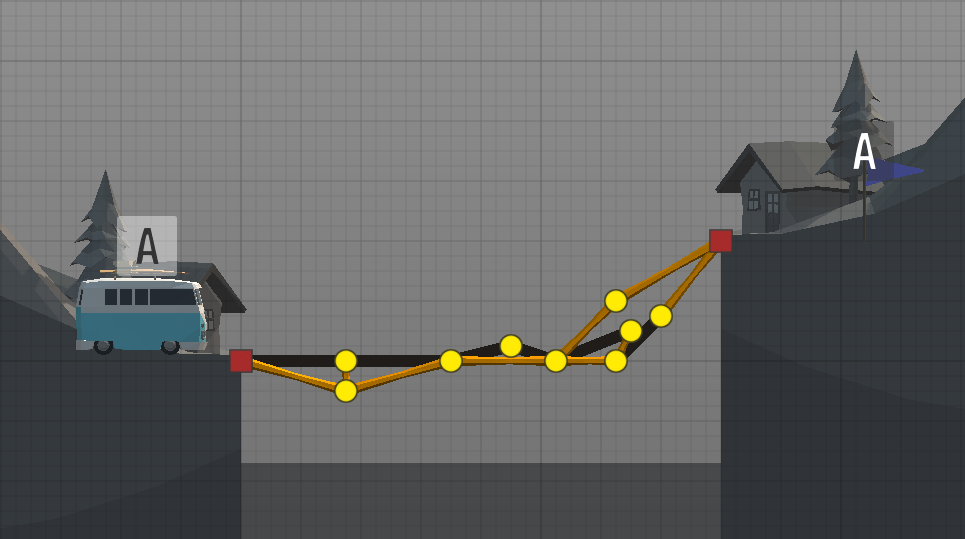
\includegraphics[width=\linewidth]{img/lvl4-poly-ea}
    \end{minipage}
    \begin{minipage}{0.32\textwidth}
        \centering
        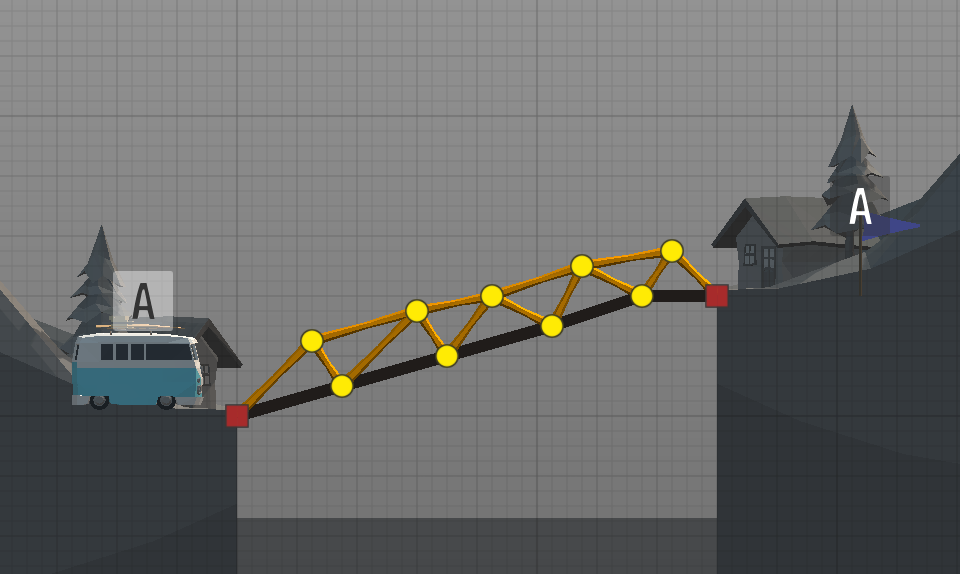
\includegraphics[width=\linewidth]{img/lvl4-poly-human}
    \end{minipage}
    \caption{Řešení čtvrté úrovně navrhnuté evolučním algoritmem. Nalevo je řešení zobrazené v simulaci, uprostřed ve hře, napravo řešení navrhnuté člověkem}
    \label{exp:lvl4}
\end{figure}


\chapter{Implementace}

V této části bakalářské práce se zaměříme na praktickou implementaci evolučních algoritmů. Kromě toho je nutné ale i implementovat fyzikální prostředí, podobné tomu jako je ve hře polybridge. V první řadě se zaměříme aby se naše simulace co nejvěrněji podobala hře, což umožní použít řešení navrhnuté evolučními algoritmy i ve hře. Následně navrhneme několik různých podob evolučního algoritmu pro stavbu mostu a ty mezi sebou porovnáme. Jako programovací jazyk jsme zvolili Python. Kompletní implementaci i se stručnou dokumentací můžeme nálezt na githubu \cite{git}.

\section{Související literatura}

Pro návrh evolučních operátorů využijeme inspiraci z existujících studií, které se zaměřili na podobný problém. Konkrétně z diplomové práce Huga Lispectora \cite{Lispector2022} adoptujeme metodu chytré inicializace mostů. Dále použijeme některé evoluční operátory z programovacího projektu autora AstroSam \cite{AstroSam2023}. Je třeba poznamenat, že obě zmíněné práce se nevěnují přesně stejnému problému, což nám znemožňuje přímé porovnání našich výsledků s těmito studiemi.

\section{Fyzikální engine}

Jako fyzikální engine pro simulaci jsme zvolili Box2D \cite{box2d}. Box2D je open-source fyzikální engine, který poskytuje simulaci pohybu objektů ve 2D prostoru. Je často využíván ve vývoji počítačových her ale také simulací a umožňuje snadné zpracování kolizí, gravitace, tuhosti objektů a dalších fyzikálních jevů. Tento engine používáme dostopnými knihnovami v Pythonu, ale původně byl implementován v~jazyce C++, což snižuje výpočtení náročnost simulace umožňuje nám iterovat přes rozsáhlé množství simulací. Pro tento engine jsme se rozhli jelikož z dostupných zdrojů víme, že stejný engine použili i vývojáři hry Poly Bridge \cite{Reddit}. 

\section{Aproximace hře Poly Bridge}

V naší simulaci jsme implementovali různé aspekty hry pomocí následujících komponent knihovny Box2D \cite{b2docs}:

\begin{itemize}
    \item \emph{Materiály}: Ty jsou modelovány jako dynamické objekty, pro které používáme \texttt{Box2D.b2DynamicBody}.
    \item \emph{Klouby}: Pro spoje různých materiálů jsme využili \texttt{Box2D.b2RevoluteJoint}.
    \item \emph{Zátež na prvky}: Abychom zjistili síly působící na jednotlivé elementy v simulaci, používáme metodu \texttt{b2body.GetReactionForce()}, která vrací reakční sílu vzniklou v důsledku interakce těles.
\end{itemize}

\subsection{Testy}

Abychom v naší simulaci co nejvěrněji napodobili chování fyzikálních prvků jako ve hře, zavedli jsme šest různých testů. Tyto testy zkoumají aspekty fyzikální simulace, jako jsou odolnost materiálů v proměnlivých podmínkách, hmotnost materiálů a interakci sil mezi objekty.

Zvolené testy jsou následující:

\begin{enumerate}
    \item \textbf{2 vozovky mezi dvěma pevnými body} Očekávaným výsledkem je, že konstrukce praskne pod zatížením samotných vozovek.
    \item \textbf{6 dřevěných dílů mezi dvěma pevnými body} Očekáváme, že konstrukce vydrží bez prasknutí.
    \item \textbf{7 dřevěných dílů mezi dvěma pevnými body} V tomto testu očekáváme, že konstrukce pod tíhou praskne.
    \item \textbf{Symetrický obrazec z 13.66 metrů vozovky, zavěšený na jednom kusu vozovky} Testujeme, zda vozovka unese zatížení bez prasknutí.
    \item \textbf{Symetrický obrazec z 14.66 metrů vozovky, zavěšený na jednom kusu vozovky} V tomto případě testujeme, zda konstrukce nevydrží zatížení a praskne.
    \item \textbf{Komplexní most z vozovek a dřeva, po kterém přejede auto} Cílem tohoto testu je prozkoumat interakci sil mezi různými materiály, kdy očekáváme, že most vydrží přejetí auta.
\end{enumerate}

Vizualizaci testů můžeme vidět na obrázku \ref{impl-fig:1}

\begin{figure}[ht]
    \centering
    \begin{minipage}{0.49\textwidth}
        \centering
        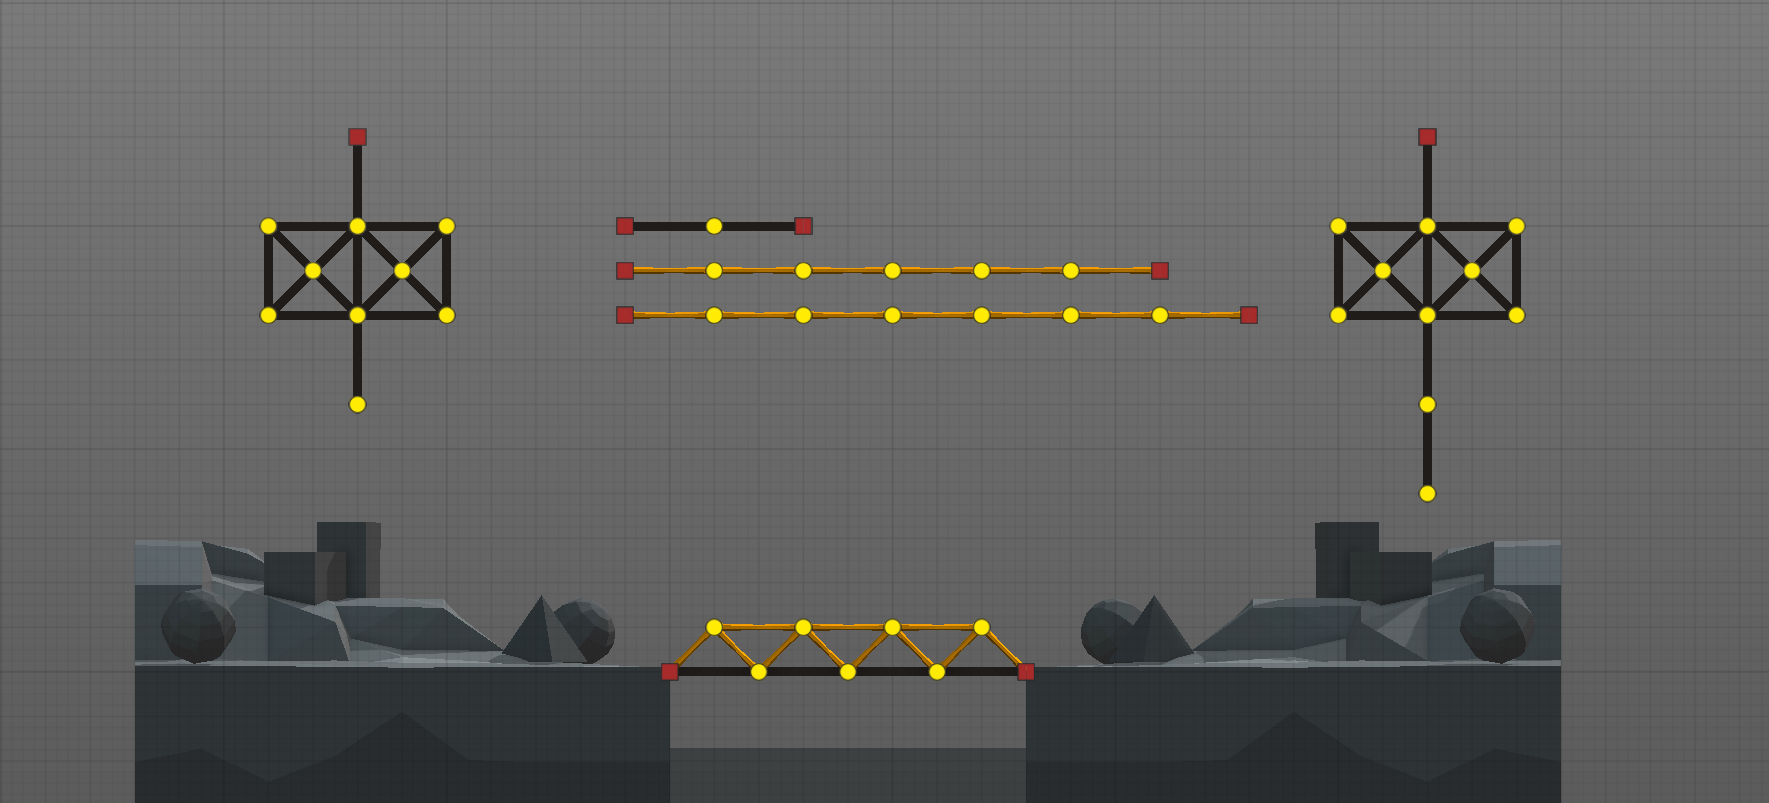
\includegraphics[width=\linewidth]{img/poly_tests.png}
    \end{minipage}\hfill
    \begin{minipage}{0.49\textwidth}
        \centering
        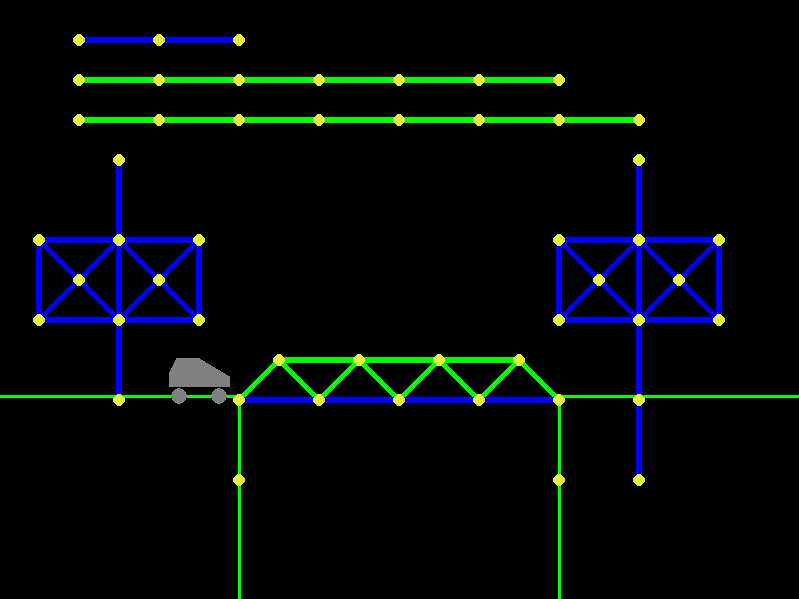
\includegraphics[width=\linewidth]{img/sim_tests.png}
    \end{minipage}
    \caption{Vizualizace testů ve hře polybridge (vlevo) a v simulaci (vpravo). Test č.1 nahoře uprostřed. Test č. 2 a 3 pod test č.1. Nalevo test č.4. Napravo test č.5. Most z 6. testu uprostřed. Vozidlo jede z levého břehu na pravý}
    \label{impl-fig:1}
\end{figure}

Naše implementace simulace ma $4$ různé parametry.
\begin{itemize}
    \item \emph{Hustota dřeva}: Hustota materiálů pro dřevo (\texttt{Box2D.b2Density}).
    \item \emph{Koeficient hustoty}: Násobek hustoty dřeva, který bude použit pro hustotu vozovky.
    \item \emph{Max. zatížení dřeva}: Maximální zatížení dřeva.
    \item \emph{Keoficient zatížení}: Násobek maximálního zatížení dřeva, který bude použit pro maximální zátížení vozovky.
\end{itemize}

Pro nalezení takových parametrů, které splní nejvíce testů jsme zvolili \textit{Random search} \cite{Random}. Prohledaná rozmezí těchto parametrů a jejich nejlepší nalezené hodnoty můžeme vidět v tabulce \ref{tab:1}. Bohužel se nám nepodařilo najít takové parametry, abychom splnili všechny. Rozhodli jsme se že $5.$ test vyřadíme.


\begin{table}[b!]
\centering
\begin{tabular}{l@{\hspace{1.5cm}}D{.}{,}{3}D{.}{,}{3}}
\toprule
\textbf{Parametr} & \multicolumn{1}{c}{\textbf{Rozmezí}} & \multicolumn{1}{c}{\textbf{Nalezená hodnota}$^a$} \\
\midrule
\emph{Hustota dřeva} & [0,01-3,01] & 1,348 \\
\emph{Max. zatížení dřeva} & [50,0-2050,0] & 765,0 \\
\emph{Koeficient hustoty} & [0,3-9,3] & 3,992 \\
\emph{Koeficient zatížení} & [0,1-5,1] & 0,821 \\
\bottomrule
\end{tabular}
\caption{Parametry pro simulaci, prohledávaná rozmezí a jejich nejlepší nalezená hodnoty.}\label{tab:1}
\footnotesize \textit{Pozn: $^a$Zaokrouhleno na 3 desetinná místa}
\end{table}


\subsection{Úrovně}

Jako testovací prostředí pro evoluční algoritmus jsme zvolili první $4$ úrovně z původní hry (viz obrázky \ref{impl-fig:2}, \ref{impl-fig:3}, \ref{impl-fig:4} a \ref{impl-fig:5}). Více úrovní jsme kvůli jejich komplexitě nezahrnuli.

\begin{figure}[ht]
    \centering
    \begin{minipage}{0.49\textwidth}
        \centering
        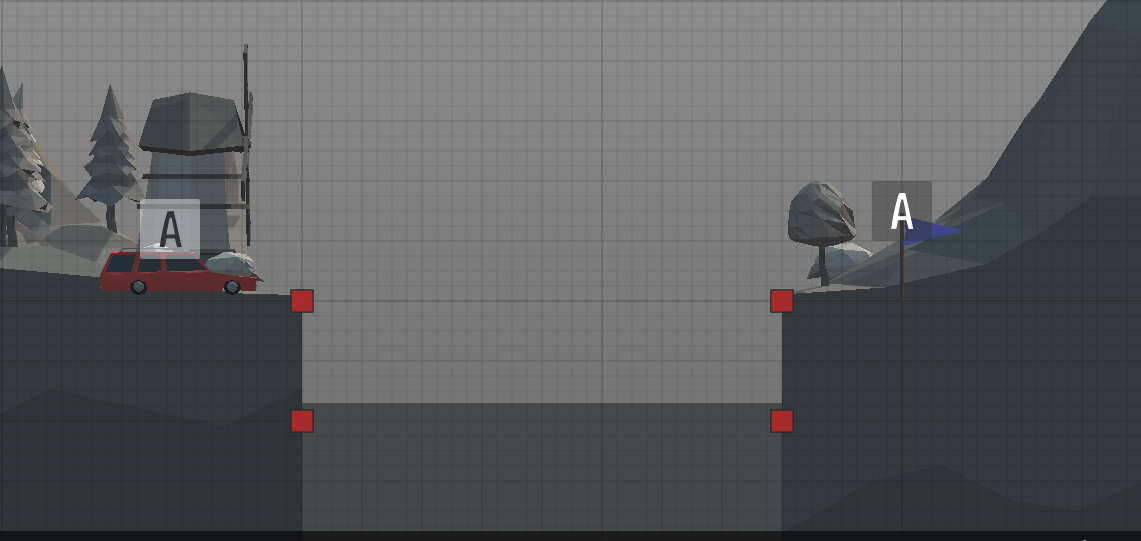
\includegraphics[width=\linewidth]{img/poly_lvl1.png}
    \end{minipage}\hfill
    \begin{minipage}{0.49\textwidth}
        \centering
        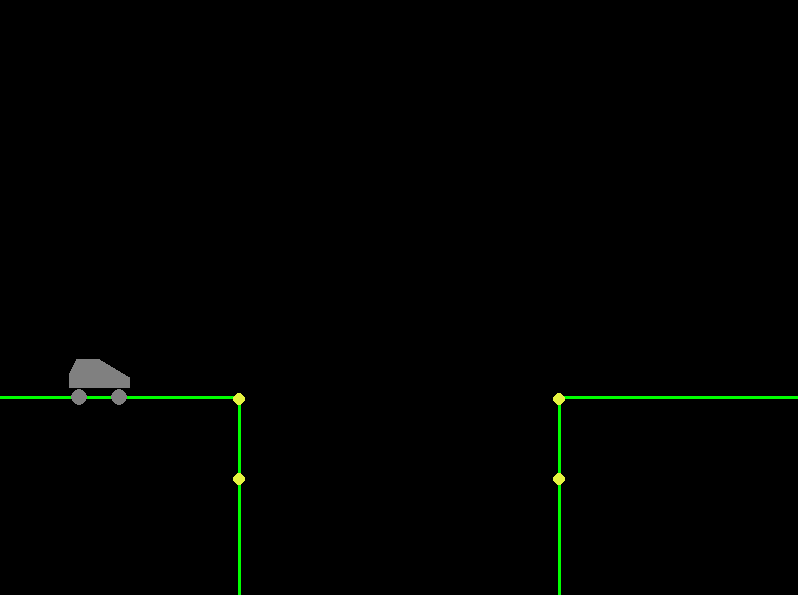
\includegraphics[width=\linewidth]{img/impl_lvl1.png}
    \end{minipage}
    \caption{Vizualizace $1.$ úrovně ve hře polybridge (vlevo) a v simulaci (vpravo)}
    \label{impl-fig:2}
\end{figure}

\begin{figure}[ht]
    \centering
    \begin{minipage}{0.49\textwidth}
        \centering
        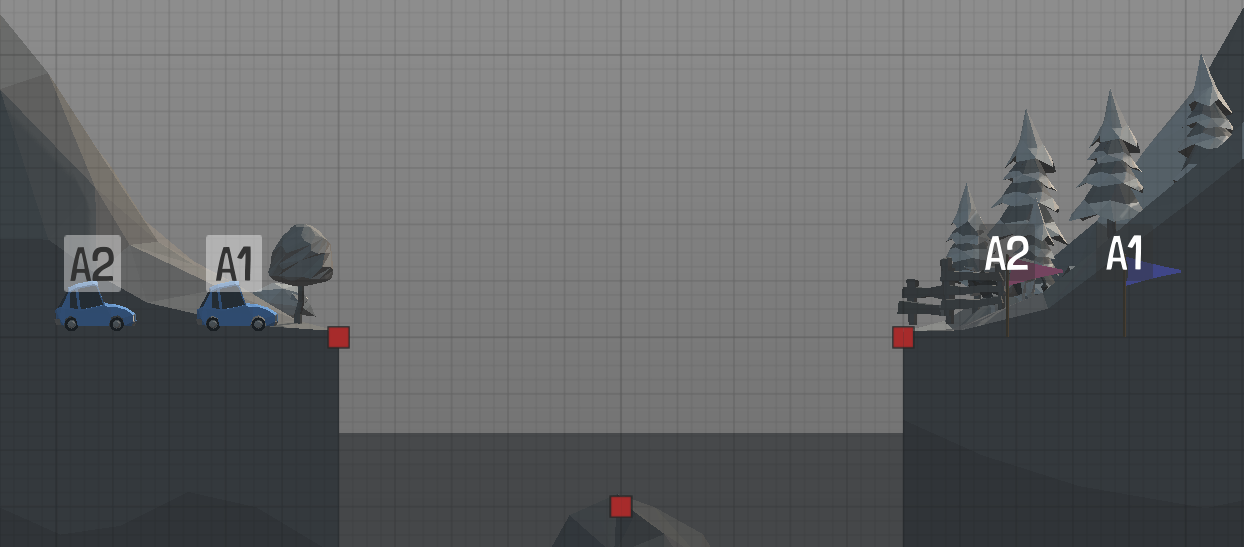
\includegraphics[width=\linewidth]{img/poly_lvl2.png}
    \end{minipage}\hfill
    \begin{minipage}{0.49\textwidth}
        \centering
        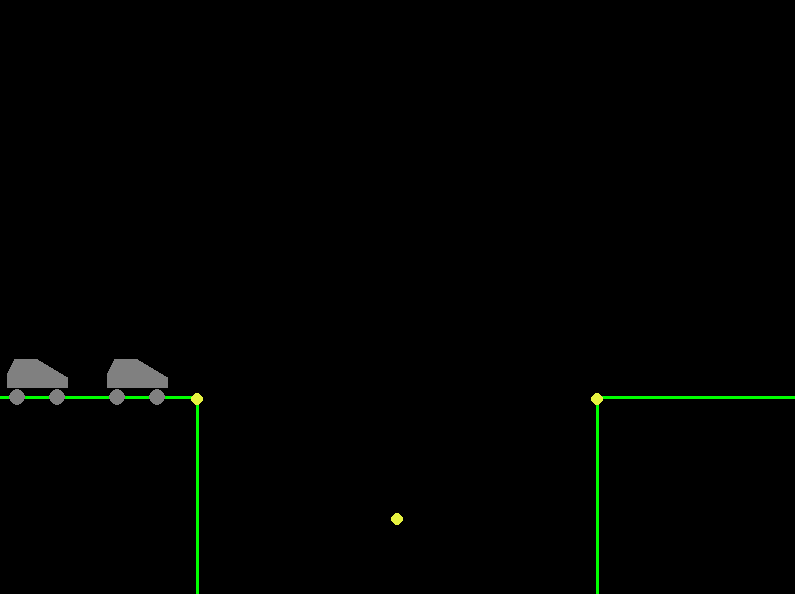
\includegraphics[width=\linewidth]{img/impl_lvl2.png}
    \end{minipage}
    \caption{Vizualizace $2.$ úrovně ve hře polybridge (vlevo) a v simulaci (vpravo)}
    \label{impl-fig:3}
\end{figure}

\begin{figure}[ht]
    \centering
    \begin{minipage}{0.49\textwidth}
        \centering
        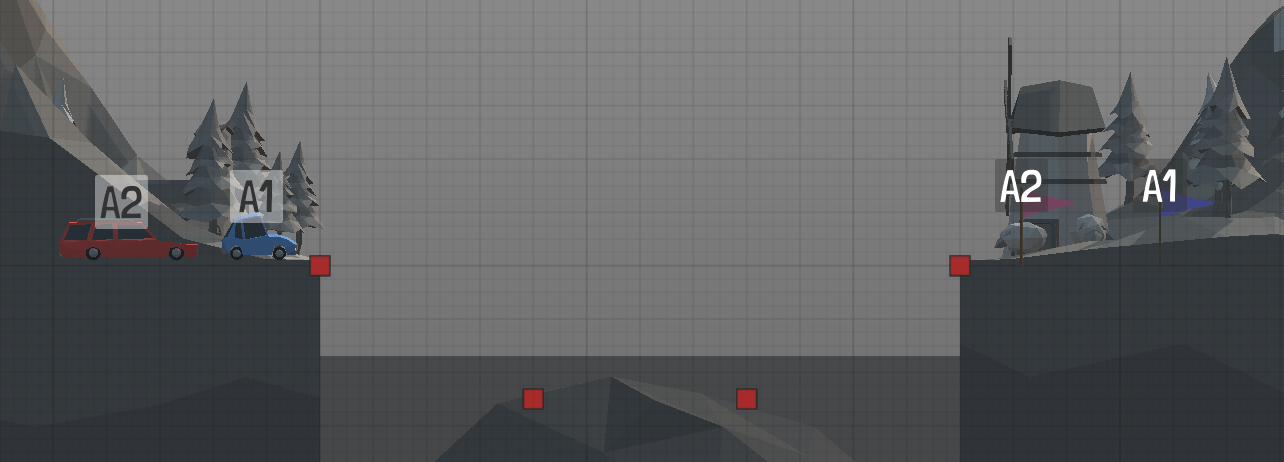
\includegraphics[width=\linewidth]{img/poly_lvl3.png}
    \end{minipage}\hfill
    \begin{minipage}{0.49\textwidth}
        \centering
        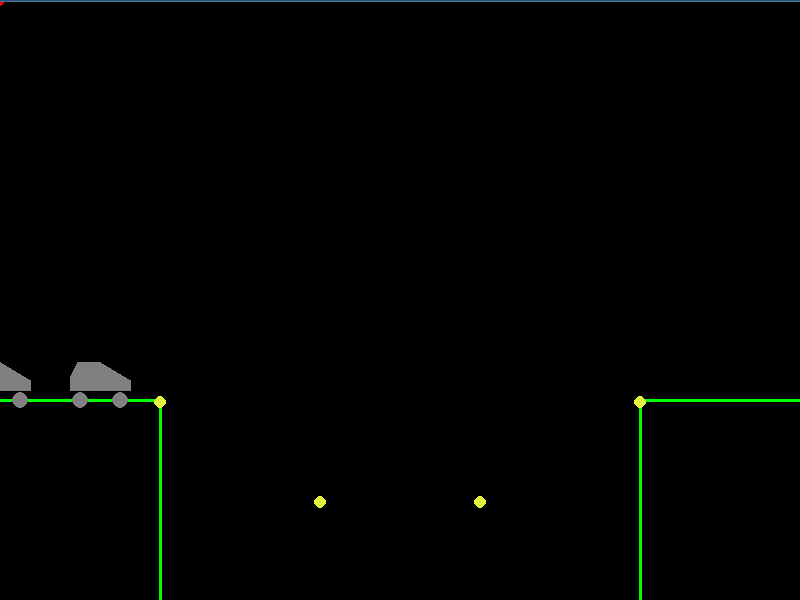
\includegraphics[width=\linewidth]{img/impl_lvl3.png}
    \end{minipage}
    \caption{Vizualizace $3.$ úrovně ve hře polybridge (vlevo) a v simulaci (vpravo)}
    \label{impl-fig:4}
\end{figure}

\begin{figure}[ht]
    \centering
    \begin{minipage}{0.49\textwidth}
        \centering
        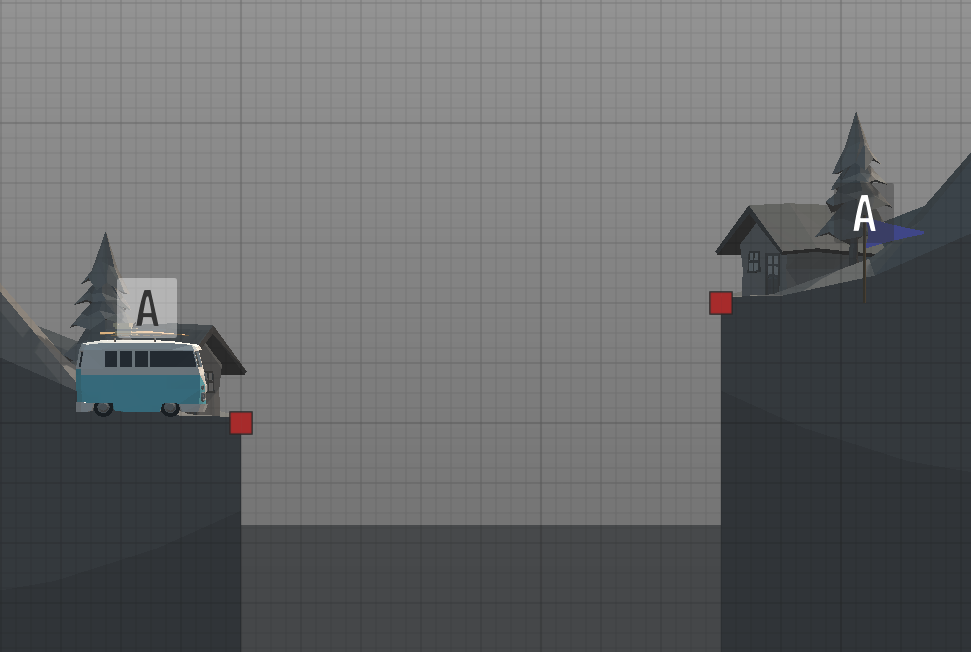
\includegraphics[width=\linewidth]{img/poly_lvl4.png}
    \end{minipage}\hfill
    \begin{minipage}{0.49\textwidth}
        \centering
        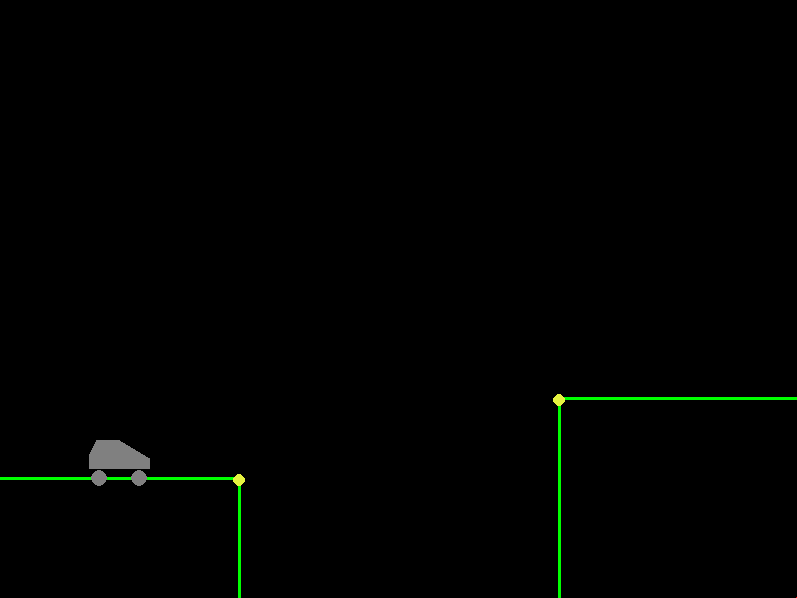
\includegraphics[width=\linewidth]{img/impl_lvl4.png}
    \end{minipage}
    \caption{Vizualizace $4.$ úrovně ve hře polybridge (vlevo) a v simulaci (vpravo)}
    \label{impl-fig:5}
\end{figure}


\section{Aplikace evolučních algoritmů}

V následující sekci ukážeme, jak jsme navrhli různé typy genetický operátorů. Budeme používa následující značení.
\begin{itemize}
    \item $l_{max}$ je maximální délka materiálu
    \item $T$ je množina všech materiálů, které můžeme použít (vozovka, dřevo, nic)
    \item $g$ je genom jedince, nebo také jeden konkrétní most
    \item $d_{min}(g)$ minimální vzdálenost vozidla od úrovní definovaného bodu na druhé straně řeky, které se podařilo dosáhnout v simulaci
    \item $cost(g)$ cena mostu $g$
\end{itemize}

Ve všech případech se snažíme optimalizovat dvě hodnoty a to jak daleko naše vozidlo dojelo a cenu mostu. V rámci algoritmu se tedy primárně snažíme maximalozovat $-d_{max}(g)$ a sekundárně $-cost(g)$.

Naše fitness funkce $f$ bude tedy udávaná dvojicí čísel. $$f(g) = (-d_{min}(g), -cost(g))$$

\subsection{Jednoduchý návrh}

Nejjednušší návrh danému problému by mohl vypadat následovně. Reprezentace genu je vektor dvojic čísel $c \in \{([0, \dots, x_{max}] \times [0, \dots, y_{max}])\}^n$ kde $x_{max} \in \N$ a $y_{max} \in \N$ je šířka a výška úrovně a vektor $t \in T^n$. Most se pak z genomu postavíme následovně. Iterujeme přes všechny dvojce z $c$ a zárověn i přes materiály z $t$. Mezi bod tvořený současnou dvojicí a posledním bodem, na který jsme metariál přidali, se snažime položit současný materiál. Pokud je současný bod od toho minulého příliš daleko tak jej přiblížíme aby jeho vzdálenost byla $l_{max}$. Na začátku jako poslední bod vybereme nejvyšší kotvu na levém břehu. Tímto způsobem se snažíme napodobit posloupnost kliknutí, které by hráč normálně provedl.

Jake mutaci jsme zvolili náhodné posunutí pozice kliknutí (bodu) o $\pm 1$ s pravděpodobností $\frac{1}{n}$ a náhodnou změnu meteriálu s pravděpodobností $\frac{1}{n}$.

Jako křížení jsme použili jednobodové křížení vektoru $c$ a $t$ podle stejně zvoleného náhodného bodu. Jako selekci jsme zvolili turnajovou selekci.

Jak můžeme vidět v experimentu \ref{exp:2}, algoritmu se nedaří stavět příliš kvalitní mosty. Domníváme se, že by tomu tak je z následujících důvodů.

\begin{itemize}
    \item Z principu reprezentace jedince je nepravděpodobné, aby vznikaly krátké hrany, které mohou být klíčové pro kvalitní řešení.
    \item I malá mutace na začátku genu může mít velký vliv na celkovou strukturu mostu.
    \item Křížení v naší reprezentaci nedává smysl.
    \item Fitness funkce nevrací dobrou zpětnou vazbu o kvalitě jedince (viz. obrázek \ref{impl-fig:6})
\end{itemize}

\subsection{Polární kódování}

Kvůli tomu, jak jsme reprezentovali jedince v předchozím návrhu, je nepravděpodobné, že budou vznikat krátké hrany, které mohou být zásadní pro dobré řešení. To, že náhodně zvolíme blízko od od posledního kliknutí je méně pravděpodobné, než že zvolíme bod daleko. Proto jsme navrhli kódování genu, kde dvojce z vektoru $c$ představují délku a úhel přidaného materiálu $c \in \{([0, l_{max}] \times [0, 2 \pi])\}^n$. Vektor $t$ zůstává stejný jako v předchozím případě.

Jake mutaci jsme zvolili přepsání hodnoty z $c$ na novou náhodně zvolenou s pravděpodobností $\frac{1}{n}$ a náhodnou změnu meteriálu s pravděpodobností $\frac{1}{n}$.

Křížení a selekci použijeme stejnou jako v předchozím případě.

\subsection{Vylepšená fitness funkce}

Jedním z problémů, se kterým se náš současný návrh potýká je ten, že naše fitness funkce moc dobře nerozlišuje, jak je dané řešení kvalitní. Na obrázku \ref{impl-fig:6} můžeme vidět dva různé jednice, kteří mají stejnou fitness, a v kvalitě se značně liší.


\begin{figure}[ht]
    \centering
    \begin{minipage}{0.49\textwidth}
        \centering
       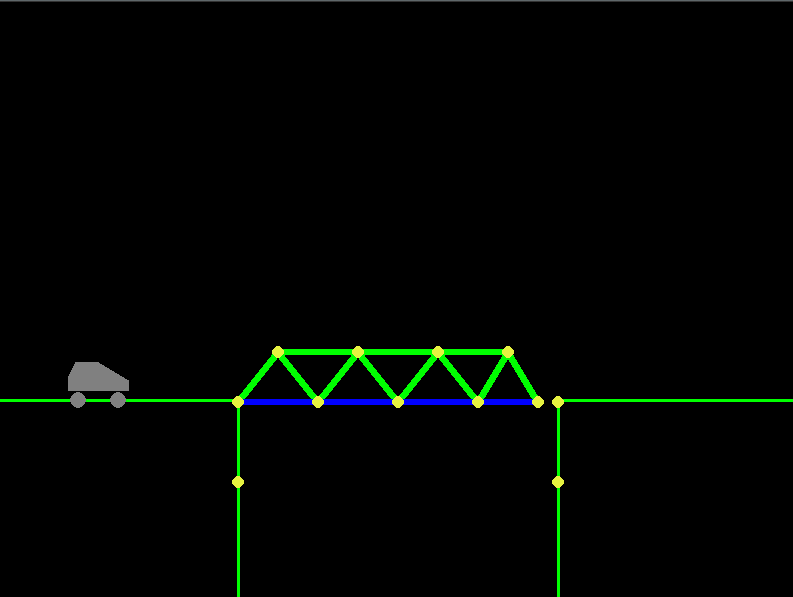
\includegraphics[width=\linewidth]{img/almost_good_bridge.png}
    \end{minipage}\hfill
    \begin{minipage}{0.49\textwidth}
        \centering
        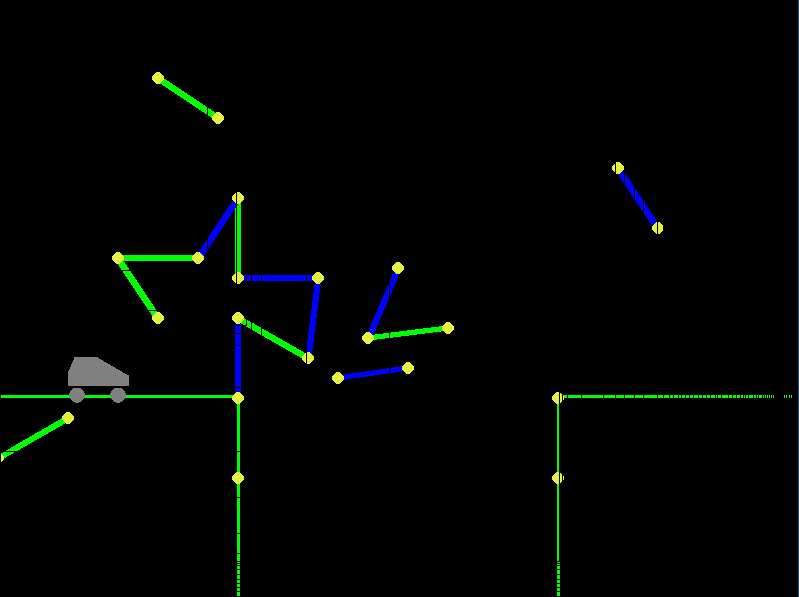
\includegraphics[width=\linewidth]{img/bad_bridge.png}
    \end{minipage}
    \caption{Dva mosty se stejnou fitness, ale rozdílných kvalit}
    \label{impl-fig:6}
\end{figure}

Navrhli jsme proto dvě různé penalizace, které můžeme do fitness zapojit.

\begin{itemize}
    \item Penalizace za umisťování materiálů, který se nespojí s další materiálem. Lépe propojený most by měl mít lepší stabilitu.
    \item Penalizace za všechny kotvy, které jedinec nepoužil. V praxi použijem vzdálenost každého kliknutí ke všem nepoužitým kotvám. Most který používá více kotev by měl být stabilnější.
\end{itemize}

Nová fitness funkce pak vypadá následovně. $$f(g) = (-d_{min}(g) + \alpha \cdot mat + \beta \cdot anch, -cost(g))$$ Koeficinety $\alpha, \beta \in \R$ značí váhu penalizace a $mat, anch$ jsou hodnoty penalizace za nespojený materiál a nevyužité kontvy.

Použijeme stejnou selekci, mutaci a reprezentaci jedince jako v předchozím návrhu.

\subsection{Měnící se fitness}

V rámci našeho přístupu jsme narazili na specifický problém spojený se stabilitou mostu. Spočívá v tom, že dokud není most zcela dokončen, nedosahuje potřebné stability, které je potřeba pro přejetí vozidlem. Abychom se s tímto omezením vypořádali, rozhodli jsme se pro zjednodušení problému a využití techniky zvané \emph{inkrementální evoluční alogritmus} navrhnuté ve článku Mansouryho Nashaata et al. \cite{IGA}. Na začátku experimentu proto začínáme s břehy blíže umístěnými k sobě a jakmile dosáhneme dostatečně nízké průměrné fitness v celé populaci, vzdálenost postupně zvětšujeme, dokud nedosáhneme vzdálenosti definové úrovní. 

Použijeme stejnou selekci, mutaci a reprezentaci jedince jako v předchozím návrhu.

\subsection{Grafové kódování}

V této části bychom chtěli představit odlišný způsob, jak kódovat jednotlivce. Naše dosavadní kódování značně trpí tím, že je nepravděpodobné aby, se v jednom bodě spojilo více, než dva kusy materiálu. Tento problém se pokusíme vyřešit tím, že jedince budeme kódovat jako graf, tedy pomocí vrcholů a hran. To v praxi znamená, že gen jedince se skládá z množiny vrcholů $V$, množiny hran $E \subseteq V \times V$, funkce $\sigma_v : V \rightarrow \R^2$ která je projekcí $V$ do roviny a $\sigma_e : E \rightarrow T$. Naše navržené genetické operátory vypadají následovně.

\begin{itemize}
    \item \textbf{inicializace}: Do $V$ přidáme všechny kotvy z úrovně. Náhodně vybereme materiál $t \in T$, vrchol $v_1 \in V$, úhel $\varphi$ a délku $0 < l < l_{max}$. Vytvoříme nový vrchol $v_2$ a vložíme jej do $V$. Upravíme $\sigma_v$ tak, že $v_2$ se promítne na bod ve vzdálenosti $l$ a pod úhlem $\varphi$ od $\sigma_v(v_1)$. Vytvoříme novou hranu $(v_1, v_2)$ a přidáme jí do $E$ a zároveň upravíme $\sigma_e$ tak, že $\sigma_e((v_1, v_2)) = t$. Opakujeme dokud nevytvoříme $n$ nových vrcholů. Následně náhodně volíme dva vrcholy $v_1, v_2 \in V$. Pokud $||\sigma_v(v_1) - \sigma_v(v_2)|| < l_{max}$ vytvoříme novou hranu $(v_1, v_2)$ a přidáme do $E$. Upravíme $\sigma_e((v_1, v_2)) = t$ pro náhodně zvolené $t \in T$. Opakujeme $2n$-krát.
    \item \textbf{mutace}: Budeme rozlišovat mutaci pro vrcholy a mutaci pro hrany. Mutace pro vrcholy upraví $\sigma_v$ tak, že projekci vrcholu $v \in V$ přemístí na náhodně zvolený bod z $\{ x \in \R^2 | \forall v_2 \in Adj(v_1), ||x - \sigma_v(v_2)|| < l_{max}\}$ kde $Adj(v_1) = \{v \in V | (v_1, v) \in E\}$. Jinými slovy náhodně posumeme vrchol $v$ tak, aby nebyl příliš daleko od žádného vrcholu s nímž byl $v$ spojen hranou. Mutace pro hrany může hranu přidat, odebrat jí nebo změnit $\sigma_e$ náhodné hrany na jiný typ materiálu.
    \item \textbf{křížení}: Dva jedince můžeme skřížit následovně. Nechť $V_1, E_1$ je množina všech vrcholů a hran prvního z rodičů a $V_2, E_2$ druhého. Nechť $\sigma_{v_p}$ je spojení $\sigma_v$ funkcí obou rodičů a $\sigma_{e_p}$ spojení $\sigma_e$ funkcí obou rodičů. Zvolíme náhodně hranici $min\{\sigma_{v_p}(v)_x | v \in V_1 \cup V_2\} < p_x < max\{\sigma_{v_p}(v)_x | v \in V_1 \cup V_2\}$. Nechť $L = \{ v | v \in V_1, \sigma_{v_p}(v)_1 < p_x\}$ a $R = \{ v | v \in V_2, \sigma_{v_p}(v)_1 > p_x\}$. Vrcholy genu potomka pak budou z $V_p = R + L$ a hrany $E_p = (E_1 + E_2) \cap V_p \times V_p$, kterým navíc přidáme všechny $(v_1, v_2), v_1 \in R, v_2 \in L, ||\sigma_{v_p}(v_1) - \sigma_{v_p}(v_2)|| < l_{max}$ s pravděpodobností $\alpha$. $\sigma_v$ potomka bude $\sigma_{v_p}$ a stejně tak pro $\sigma_e$. Příklad takové mutace můžeme vidět na obrázku \ref{impl-fig:8}
\end{itemize}

\begin{figure}[ht]
    \centering
    \begin{minipage}{0.24\textwidth}
        \centering
        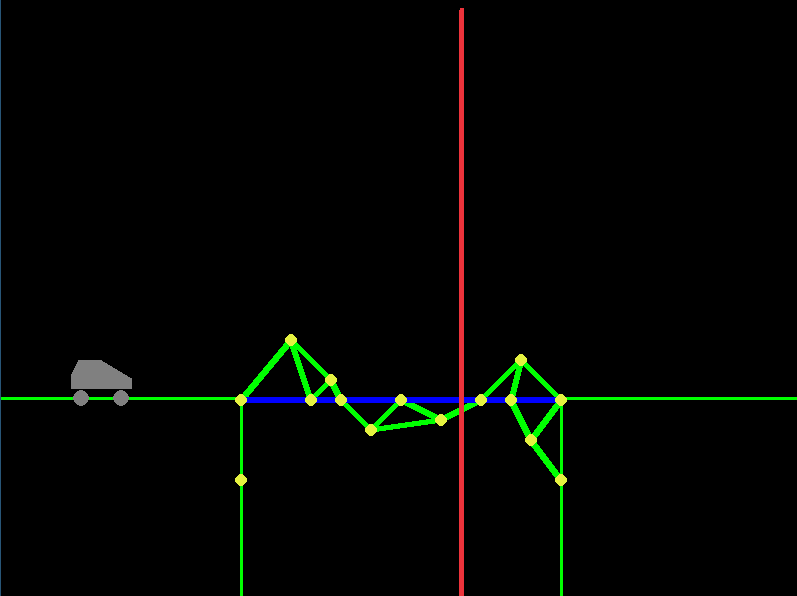
\includegraphics[width=\linewidth]{img/bridge_p1.png}
    \end{minipage}\hfill
    \begin{minipage}{0.24\textwidth}
        \centering
        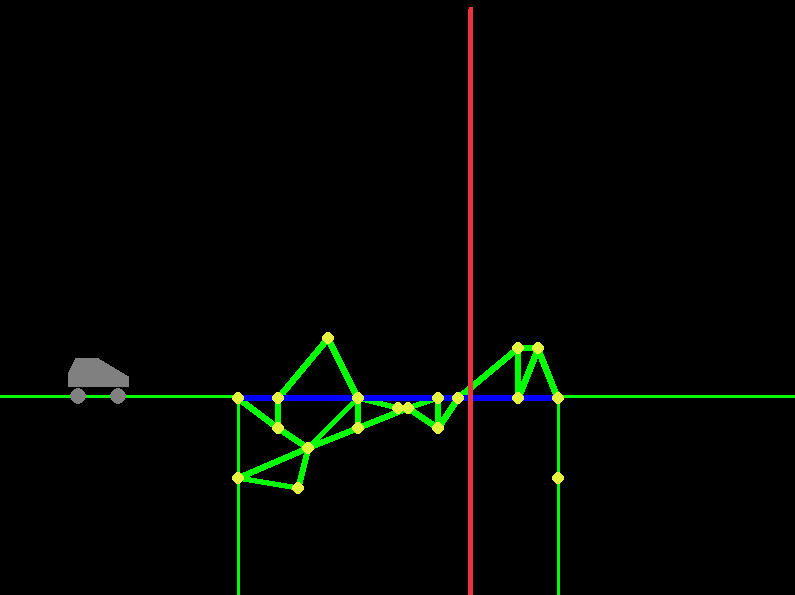
\includegraphics[width=\linewidth]{img/bridge_p2.png}
    \end{minipage}
    \begin{minipage}{0.24\textwidth}
        \centering
        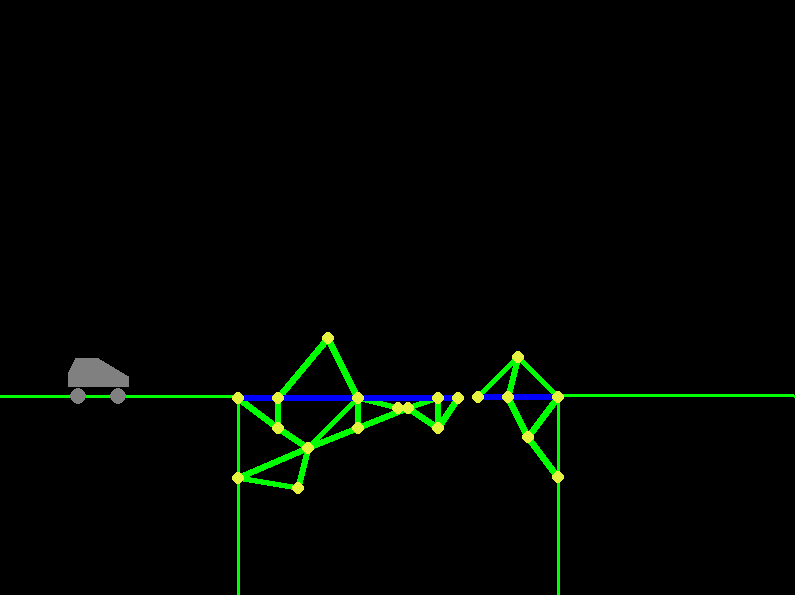
\includegraphics[width=\linewidth]{img/bridge_crossed.png}
    \end{minipage}
    \begin{minipage}{0.24\textwidth}
        \centering
        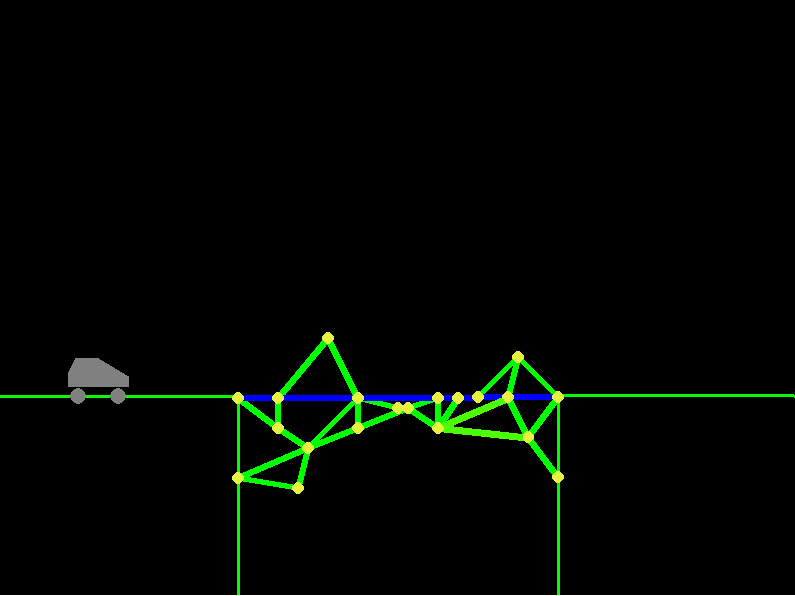
\includegraphics[width=\linewidth]{img/bridge_sups.png}
    \end{minipage}
    \caption{Příklad křížení dvou rodičů. Na 1. a 2. obrázku zleva jsou rodiče. Hranice pro náhodné křížení je vyznačena červenou čárou. Na 2. obrázku zprava křížení částí mosty. Na nejpravějším obrazku překžížení s vystužením}
    \label{impl-fig:8}
\end{figure}

Jako selekci použijeme turnajovou selekci.

\subsection{Lepší inicializace}

Do našeho algoritmu můžeme ještě zahrnout jednu z nejsilnějších techni pro evoluční algoritmy a to použití \textit{domain-specific} znalostí \cite{PASSONE2006192}. I když ještě nevíme, jak bude optimální most vypadat, dokážeme obecným způsobem navrhnout most, který sice nebude optimální, ale bude lepší, než náhodně umístěný materiál. Z tohoto důvodu jsme implementovali postup podobný tomu, který navrhli Hugo Lispector ve své diplomové práci \cite{Lispector2022}. Tento postup se skládá ze tří kroků.

\begin{enumerate}
    \item \textbf{Vytvoření vozovky}: Nejprve pro vozidlo vytvoříme vozovku a to tím způsobem, spojíme levý a pravý břeh vozovkami a náhodné délce.
    \item \textbf{Vytvoření opor}: Následně pro každou ještě nevyužitou kotvu vyberem jeden spojový kloub z předchozího kroku a spojíme je dřevěnými díly o náhodné délce.
    \item \textbf{Zpevnění}: Nakonec pro každý přidaný materiál náhodně vybereme nový bod tak, abychom jej mohli spojit jedním dílem dřeva se začátkem a koncem tohoto materiálu a navíc bod spojíme se všemi ostatními bodu v blízkém okolí s pravděpodobností $\omega$.
\end{enumerate}

Vizualizaci těchto tří kroků můžeme vidět na obrázku \ref{impl-fig:7}

\begin{figure}[ht]
    \centering
    \begin{minipage}{0.32\textwidth}
        \centering
        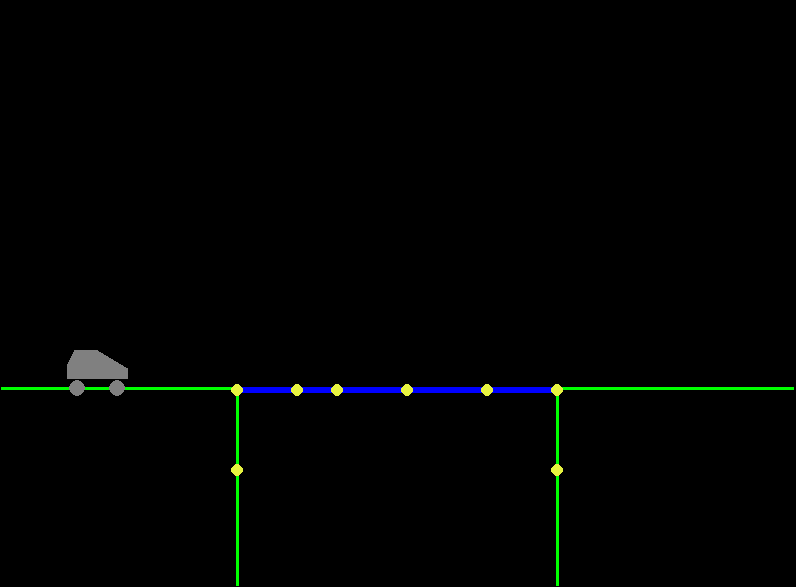
\includegraphics[width=\linewidth]{img/better_init1.png}
    \end{minipage}\hfill
    \begin{minipage}{0.32\textwidth}
        \centering
        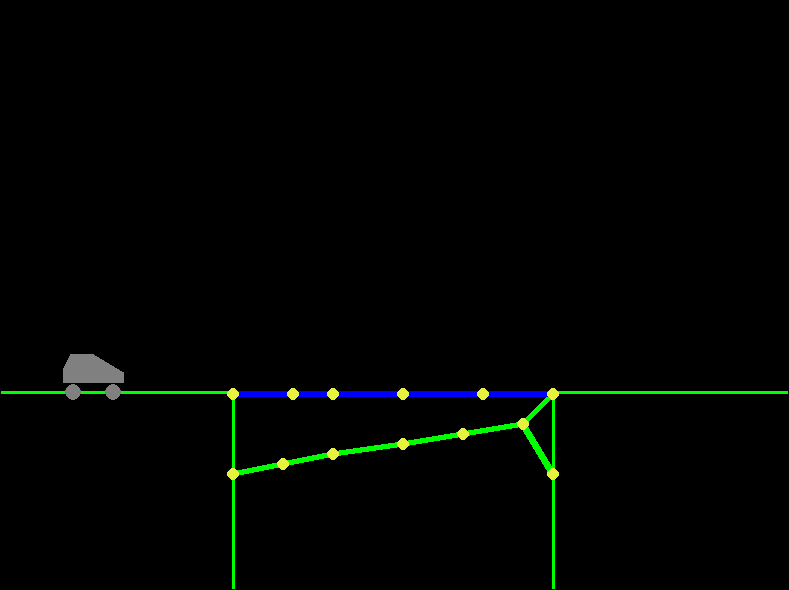
\includegraphics[width=\linewidth]{img/better_init2.png}
    \end{minipage}
    \begin{minipage}{0.32\textwidth}
        \centering
        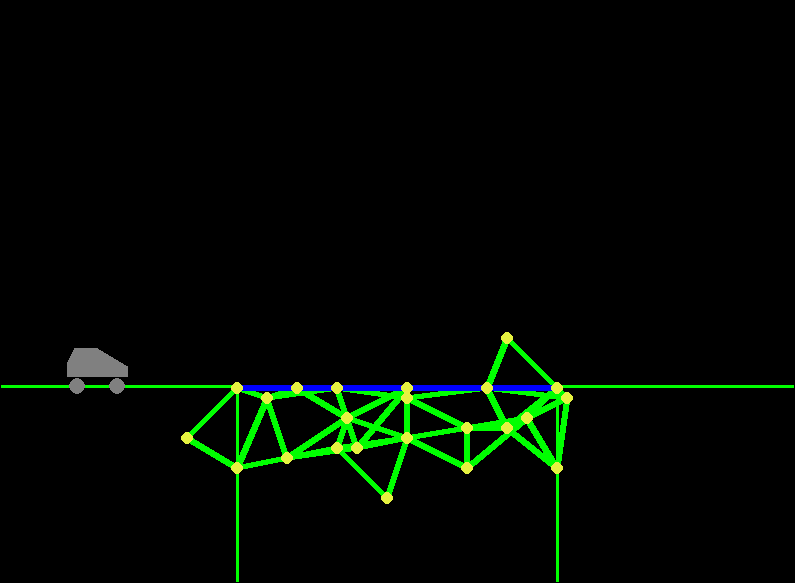
\includegraphics[width=\linewidth]{img/better_init3.png}
    \end{minipage}
    \caption{Výtváření jedince pomocí lepší inicializace. Krok \textbf{Vytvoření vozovky} vlevo, krok \textbf{Vytoření opor} uprostřed a krok \textbf{Zpevění} s $\omega = 1$ vpravo}
    \label{impl-fig:7}
\end{figure}

Použijeme selekci, křížení a mutaci z přechozího návrhu.
% Název práce v angličtině
\def\ThesisTitleEN{Evolutionary algorithms for 2D bridge construction in the Poly Bridge game}

% Jméno autora (vy)
\def\ThesisAuthor{Václav Krňák}

% Rok odevzdání
\def\YearSubmitted{2024}

% Název katedry nebo ústavu, kde byla práce oficiálně zadána
% (dle Organizační struktury MFF UK:
% https://www.mff.cuni.cz/cs/fakulta/organizacni-struktura,
% případně plný název pracoviště mimo MFF)
\def\Department{Katedra teoretické informatiky a matematické logiky}
\def\DepartmentEN{Department of Theoretical Computer Science and Mathematical Logic}

% Jedná se o katedru (department) nebo o ústav (institute)?
\def\DeptType{Katedra}
\def\DeptTypeEN{Department}

% Vedoucí práce: Jméno a příjmení s~tituly
\def\Supervisor{Mgr. Roman Neruda, CSc.}

% Pracoviště vedoucího (opět dle Organizační struktury MFF)
\def\SupervisorsDepartment{Katedra teoretické informatiky a matematické logiky}
\def\SupervisorsDepartmentEN{Department of Theoretical Computer Science and Mathematical Logic}

% Studijní program (kromě rigorozních prací)
\def\StudyProgramme{Informatika}

% Nepovinné poděkování (vedoucímu práce, konzultantovi, tomu, kdo
% vám nosil pizzu a vařil čaj apod.)
\def\Dedication{%
\xxx{Poděkování.}
}

% Abstrakt (doporučený rozsah cca 80-200 slov; nejedná se o zadání práce)
\def\Abstract{%
V této bakalářské práci se budeme zabývat řešením několika úrovní ze hry Poly Bridge pomocí umělé inteligence. Poly bridge je logická hra se sandboxovým prostředím, ve kterém je hráč veden k tomu aby postavil 2D mostní konstrukci podobnou příhradovému mostu. Hráč musí dbát na stabilitu této konstrukce, ale zároveň i na materiálovou náročnost. Vzhledem k složitosti a variabilitě problémů, které hra představuje, jsme se rozhodli použít evoluční algoritmy. Cílem práce je návrh několika genetický operátorů, které optimalizují mostní strukturu, jejich porovnání a využití mostů, které produkují, ve hře Poly Bridge.
} 

% Anglická verze abstraktu
\def\AbstractEN{%
This bachelor thesis proposes an artificial intelligence to solve several levels from the game Poly Bridge. Poly bridge is a puzzle game with a sandbox environment in which the player is led to build a 2D bridge structure similar to a truss bridge. The player has to pay attention to the stability of this structure, but also to the material requirements. Given the complexity and variability of the problems posed by the game, we decided to use evolutionary algorithms. The aim of this thesis is to design several genetic operators that optimize the bridge structure, compare them and use the bridges they produce in the game Poly Bridge. 
}

% 3 až 5 klíčových slov (doporučeno) oddělených \sep
% Hodí se pro nalezení práce podle tématu.
\def\ThesisKeywords{%
Evoluční algoritmy\sep
Polybridge\sep
Optimalizace\sep
}

\def\ThesisKeywordsEN{
Evolutionary Algorithms\sep
Polybridge\sep
Optimalization\sep
}

% Pokud některá z položek metadat obsahuje TeXové řídící sekvence, je potřeba
% dodat i verzi v obyčejném textu, která se objeví v metadatech formátu XMP
% zabudovaných do výstupního souboru PDF. Pokud si nejste jistí, prohlédněte si
% vygenerovaný soubor thesis.xmpdata.
\def\ThesisAuthorXMP{\ThesisAuthor}
\def\ThesisTitleXMP{\ThesisTitle}
\def\ThesisKeywordsXMP{\ThesisKeywords}
\def\AbstractXMP{\Abstract}

% Máte-li dlouhý abstrakt a nechceme se mu vejít na informační stranu,
% můžete použít toto nastavení ke zmenšení písma informační strany.
% (Uvažte nicméně zkrácení abstraktu, to je často lepší.)
\def\InfoPageFont{}
%\def\InfoPageFont{\small}  % odkomentujte pro zmenšení písma
\chapter{Hra PolyBridge}

Poly Bridge je logická simulovaná hra, která byla vyvinuta nezávislým vývojářským týmem Dry Cactus v roce 2016 \cite{drycactus}. Hráči mají za úkol navrhovat mosty, které musí odolat zátěži projíždějících vozidel a zároveň splňovat omezení daná rozpočtem a dostupnými materiály. Díky svému základu v realistické fyzice nabízí Poly Bridge možnost experimentovat s různými stavebními technikami a materiály.

Zajímavým aspektem hry je také komunitní prvek. Hráči mohou sdílet své vlastní návrhy mostů a úrovní online, kde je mohou ostatní hráči testovat a hodnoti. Díky tomu, je možné sdílet techniky a nápady mezi hráči z celého světa. 

\emph{\uv{Popusťte uzdu své inženýrské kreativitě v poutavém a neotřelém simulátoru stavby mostů se všemi zvonky a píšťalkami. Užijte si hodiny řešení fyzikálních hádanek v kampani a pak se vrhněte do sandboxu a vytvářejte vlastní návrhy mostů a hádanky!}} (Dry Cactus přeloženo \cite{drycactus})

\section{Vlastní hra}

Samotná hra se skládá ze 7 kampaní. V každé kampaní se nachazí 15 různých úrovní, které se postupně zvyšují v obtížnosti.

Po výběru úrovně je hráči představeno prostředí, které se ve většině případů skládají z levého a pravého břehu, řeky a jednoho nebo více vozidel. K dispozici je řada materiálů, jako je dřevo, vozovka, ocel, hydraulika a další. Materiály se od~sebe liší svou nosností, maximální délkou a cenou.

Hráč nejdříve vytvoří svůj návrh a realizuje ho klikáním na předem určené body v prostředí. Kliknutím na dva body se mezi nimi vytvoří vybraný materiál. Pokud dva materiály končí nebo začínají na stejném bodě, vytvoří se mezi nimi volně pohyblivý kloub. V každé úrovni jsou předem některé body vybrané jako kotvy. Tyto kotvy jsou nepohyblivé a hráč na ně může navázat stavbou svého mostu a získat tím oporu pro jeho výtvor.

Když je hráč se svým návrhem a realizací spokojený, může spustit simulaci. Během simulace není možné přidávat další materiály. Vozidla začnou jezdit z jedné strany mostu na druhou a hráč sleduje, zda konstrukce vydrží. Pokud most selže, hráč musí identifikovat slabá místa a provést potřebné úpravy.

Proces návrhu, testování a úprav se opakuje, dokud most nevydrží požadované zatížení bez překročení rozpočtu.

\begin{figure}[p]\centering
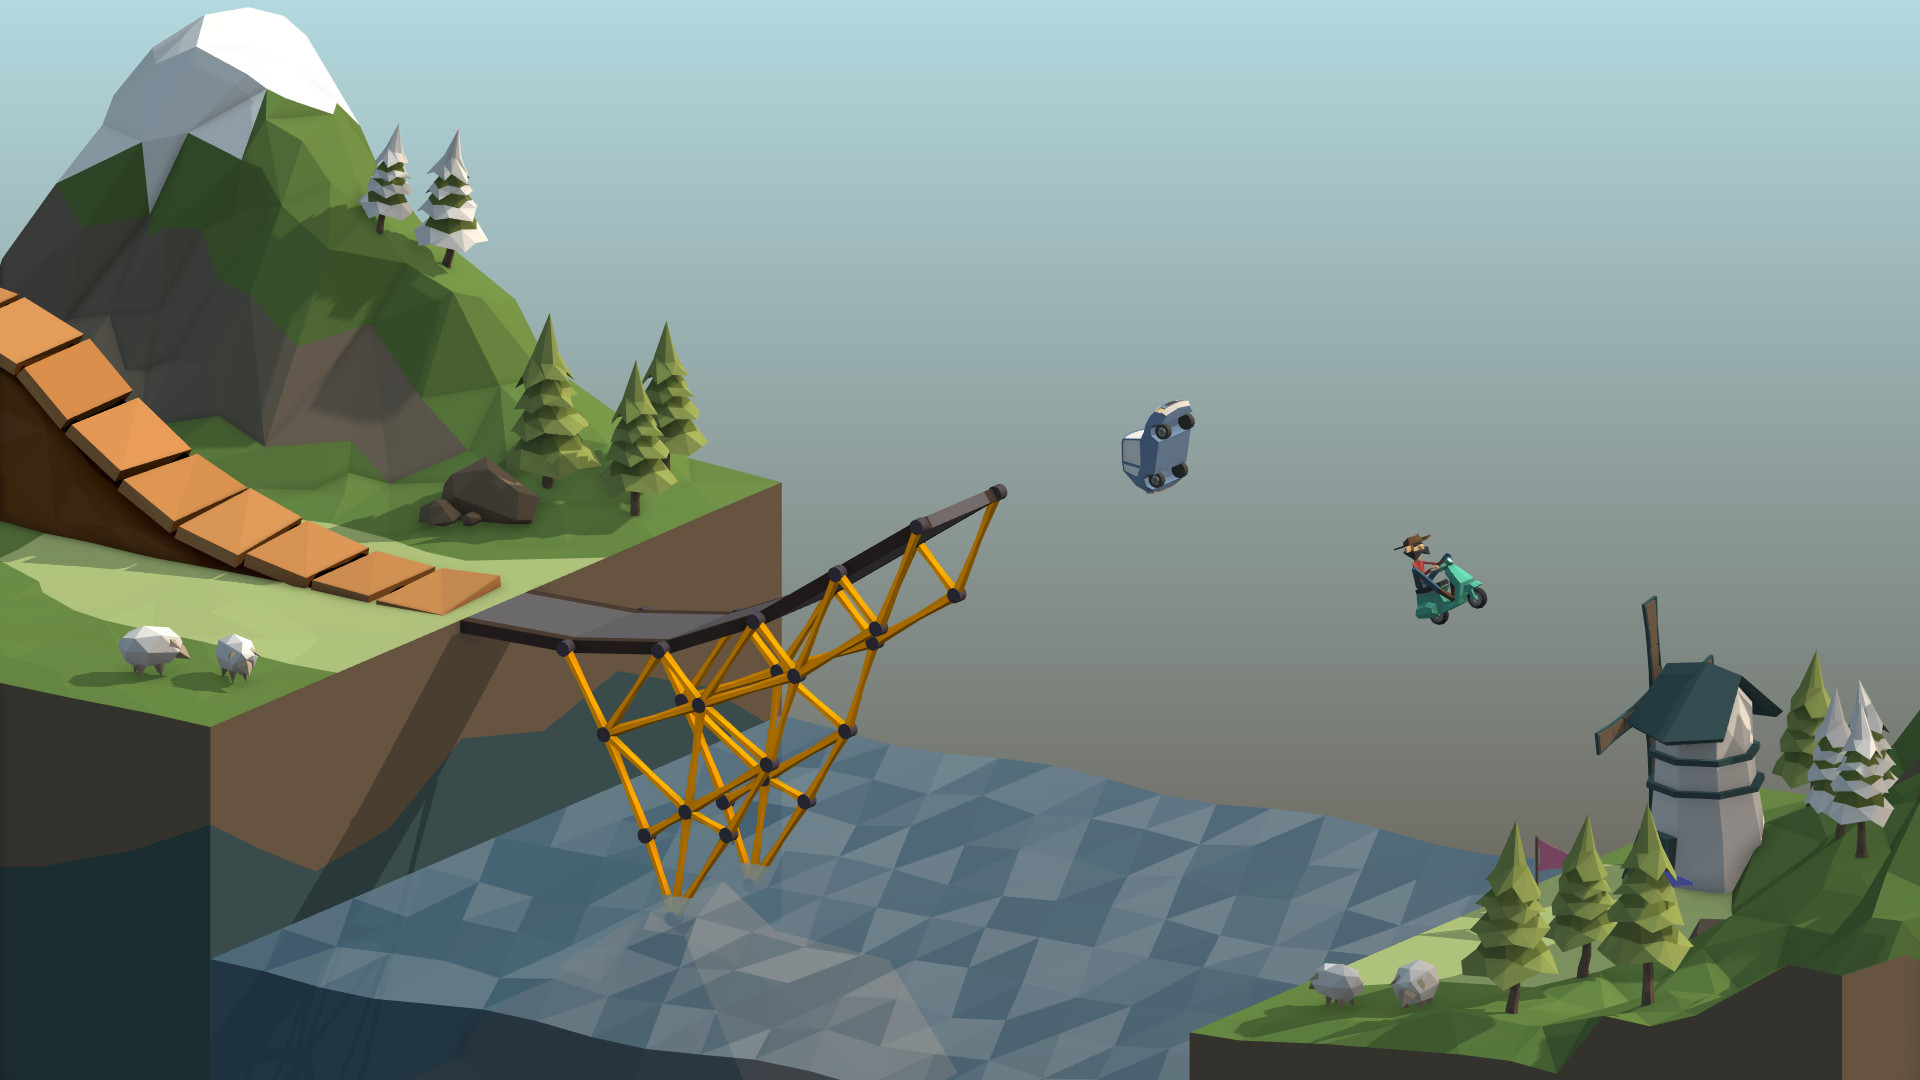
\includegraphics[width=\linewidth]{img/poly_screen_1.jpg}
\caption{Ukázka ze hry polybridge \citet{drycactus}}
\label{poly-fig:1}

\end{figure}

\begin{figure}[p]\centering
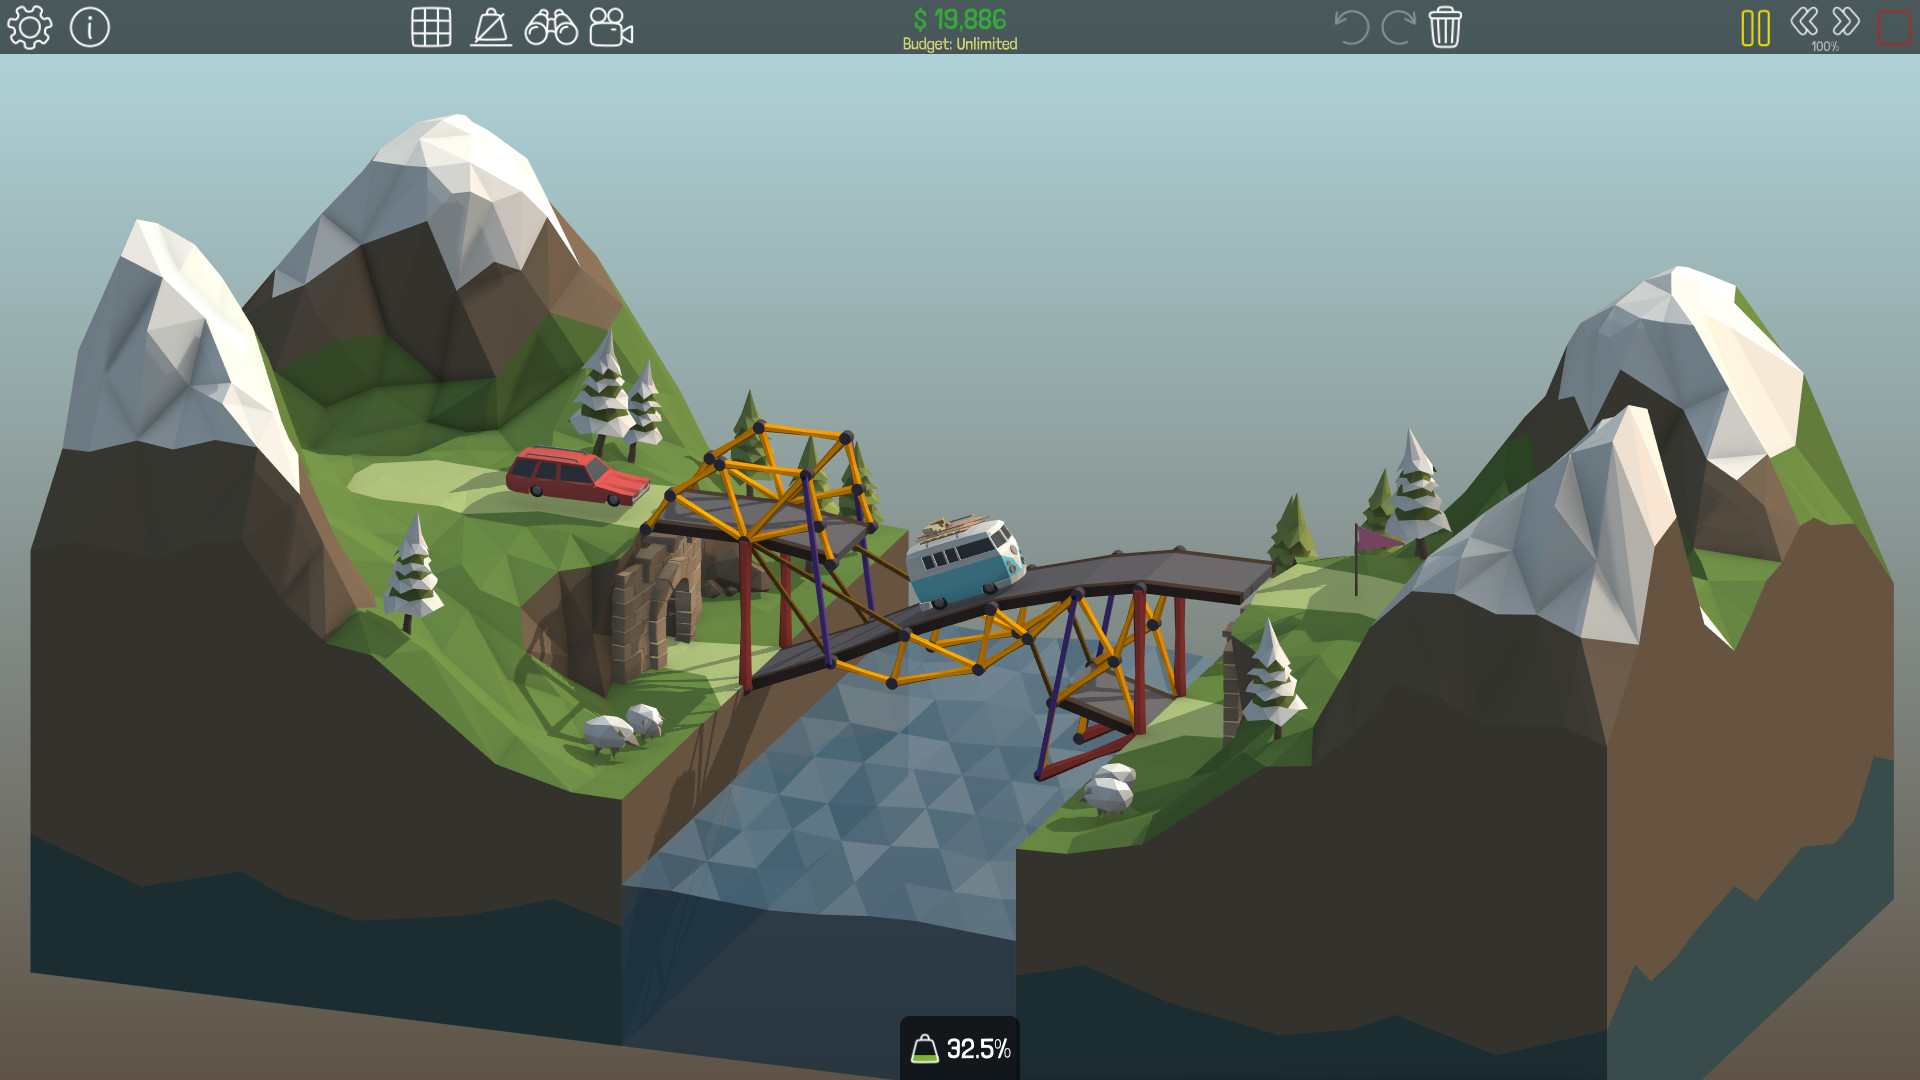
\includegraphics[width=\linewidth]{img/poly_screen_2.jpg}
\caption{Ukázka ze hry polybridge \citet{drycactus}}
\label{poly-fig:2}
\end{figure}


\chapter*{Úvod}
\addcontentsline{toc}{chapter}{Úvod}

V posledních dekádách se umělá inteligence stala klíčovým prvkem v mnoha technologických a vědeckých oborech, včetně počítačových her \cite{mnih2013playing} \cite{Vinyals2019}. Jedním z~fascinujících přístupů, jak umělá inteligence může ovlivnit interakci s počítačovými hrami, je použití evolučních algoritmů. Tyto algoritmy, inspirované biologickou evolucí, nabízejí zajímavý mechanismus pro automatizované řešení problémů a optimalizaci procesů \cite{EibenSmith2015}.

Poly Bridge je počítačová hra zaměřená na stavební inženýrství a řešení fyzikálních hádanek. Hra žádá od hráčů, aby stavěli mosty přes různé rozpětí vodních ploch s omezenými zdroji a za dodržení specifických parametrů \cite{drycactus}. Cílem této bakalářské práce je prozkoumat, jak mohou být evoluční algoritmy použity pro automatické generování a optimalizaci mostních konstrukcí v rámci hry.

Cílem této bakalářské práce je nejen prozkoumat teoretické aspekty evolučních algoritmů, ale především demonstrovat jejich praktické využití a potenciál v~kontextu moderních počítačových her. Tato práce tedy může sloužit jako příklad, jak moderní metody umělé inteligence mohou překonat tradiční přístupy používané komunitou hráčů počítačových her. 

Práce nejprve představí základní koncept evolučních algoritmů a vysvětlí jejich principy a metody. Následně bude analyzovat specifika hry Poly Bridge, aby bylo možné vytvořit fyzikální simulované prostředí pro aplikaci těchto algoritmů. Praktická část práce se zaměří na implementaci vybraných algoritmů, jejich testování a hodnocení na základě efektivity a práci se zdroji.


% Generate XMP metadata file (*.xmpdata) from thesis metadata
% The format of the xmpdata file is described in the documentation
% of the "pdfx" LaTeX package.

{
% Define \percenthack macro that expands to a literal "%" character.
% (We can use neither \char\`% nor \% as they are interpreted by TeX's
% main processor which is too late for our purposes.)
\catcode`\%=12
\global\edef\percenthack{%}
}

{
% Override some macros
\def\xxx#1{#1}
\def\sep{\string\sep\space}
\let~=\space

% Generate *.xmpdata
% It is tempting to use LaTeX's filecontents environment, but it does not
% expand macros. We need to dive deeper...
\newwrite\xmp
\immediate\openout\xmp=\jobname.xmpdata
\immediate\write\xmp{\percenthack\space Generated automatically from metadata.tex, please don't edit here.}
\def\xmpitem#1#2{\immediate\write\xmp{\string#1{#2}}}
\xmpitem\Author\ThesisAuthorXMP
\xmpitem\Title\ThesisTitleXMP
\xmpitem\Keywords\ThesisKeywordsXMP
\xmpitem\Subject\AbstractXMP
\xmpitem\Publisher{Charles University}
\immediate\closeout\xmp
}
\chapter{Závěr}

\addcontentsline{toc}{chapter}{Závěr}


V této bakalářské práci jsme zkoumali možnosti využití evolučních algoritmů pro konstrukci mostů ve hře Poly Bridge. Práce ukázala teoretický základ evolučních algoritmů a aplikuje tyto principy na specifické problémy hry. Bylo vytvořeno fyzikální prostředí schopné simulovat chování mostů. Navrhli jsme a implementovány různé genetické operátory, které byly následně testovány pro tvorbu a optimalizaci mostových struktur.

Experimentální výsledky ukázaly, že přístup založený na evolučních algoritmech je schopný efektivně generovat funkční mostní konstrukce, které nejenže splňují požadavky dané úrovně hry, ale často jsou nákladově efektivnější ve srovnání s konstrukcemi vytvořenými člověkem. Bohužel, kvůli naší nepřesné simulaci fyzkálního prostředí nebylo možné použít všechna řešení i ve hře.

Existuje několik možností, jak bychom mohli vylepšit celkové výsledky našich experimentů. Jednou z cest je zdokonalení fyzikální simulace, kterou využíváme. Toho bychom mohli dosáhnout například rozšířením a zpřesněním sady testů nebo experimentováním s různými komponentami enginu Box2D.

Také by bylo užitečné prozkoumat další metody umělé inteligence, jako je zpětnovazební učení, neuronové sítě nebo techniku zvanou \emph{novelty search} \cite{lehman2011}, které by mohly přinést nové perspektivy a vylepšení našeho výzkumu. 

